\documentclass{article}

\usepackage[preprint]{neurips_2025}


\usepackage[utf8]{inputenc} % allow utf-8 input
\usepackage[T1]{fontenc}    % use 8-bit T1 fonts
\usepackage{hyperref}       % hyperlinks
\usepackage{url}            % simple URL typesetting
\usepackage{booktabs}       % professional-quality tables
\usepackage{amsfonts}       % blackboard math symbols
\usepackage{microtype}      % microtypography
\usepackage{xcolor}         % colors


\usepackage{amsmath,amssymb,amsthm,mathtools,bm}

\theoremstyle{plain}
\newtheorem{theorem}{Theorem}
\newtheorem{proposition}{Proposition}
\newtheorem{lemma}{Lemma}
\newtheorem{corollary}{Corollary}
\theoremstyle{definition}
\newtheorem{definition}{Definition}
\newtheorem{assumption}{Assumption}
\theoremstyle{remark}
\newtheorem{remark}{Remark}

\newcommand{\ip}[2]{\left\langle#1,#2\right\rangle}
\newcommand{\softmax}{\mathrm{softmax}}
\newcommand{\rms}{\mathrm{rms}}


\title{Attention Sinks Induce Gradient Sinks}
\author{
    Yihong Chen \\
    Department of Electronic Engineering\\
    Tsinghua University\\
    Beijing, China \\
    \texttt{chenyihong@tsinghua.edu.cn} \\
    \And
    Quanming Yao \\
    Department of Electronic Engineering\\
    Tsinghua University\\
    Beijing, China \\
    \texttt{qyaoaa@tsinghua.edu.cn} \\
}


\begin{document}
\maketitle

\begin{abstract}
Attention sinks and massive activations are two recurring and closely related phenomena in Transformer models. Existing studies have largely focused on the forward pass, making it unclear whether the connection between attention sinks and massive activations is direct or mediated by a training-time mechanism. We study this question from the perspective of backpropagation. Empirically and theoretically, we show that under causal mask, attention sinks induce a pronounced concentration of gradients, which we term gradient sinks. Furthermore, in pre-norm architectures with RMSNorm, massive activations can be understood as an adaptive response to this localized gradient pressure during training. To test this hypothesis, we introduce V-scale, a modification that adjusts value-path backpropagated gradients while keeping forward behavior largely unchanged. In pretrained models with V-scale, attention sinks are preserved whereas massive activations are substantially suppressed. These findings support the view that gradient sink is a key training-time mediator linking attention sinks and massive activations.
\end{abstract}

\section{Introduction}
% 1. 引入背景与概念介绍
% 2. 当前工作介绍
% 3. 为什么当前工作不能解决我的问题
% 4. 我做了什么，提出了什么
% 5. 我如何验证
% 6. 提出本文的contribution
Understanding mechanisms of Transformer-based large language models (LLMs) becomes increasingly important. 
Two prominent and frequently co-occurring phenomena in LLMs are \emph{attention sinks} (AS), where a small number of tokens attract disproportionate attention mass \citep{xiao2024streamingllm,gu2025when,guo2025activedormant}, and \emph{massive activations} (MA), where activation magnitudes become unusually large on a small set of tokens and features \citep{bondarenko2023quantizable,sun2024massive,an2025systematic}. They are most commonly observed on the first token especially in pre-norm LLMs.

These phenomena have attracted lots of research interest. 
First, a line of work treats AS as exploitable structure that can support efficient or long-context inference \citep{xiao2024streamingllm,su2025kvsink,liu2026sinktrack} and fine-tuning \citep{liu2025all,fu2026attention,liu2026surgery}. 
Second, structural work studies how to migrate or reshape these phenomena by attention or normalization variants \citep{henry2020qknorm,miller2023attention,kaul2025from,zuhri2025softpick,qiu2025gated,bu2025valuestategated,sun2026spike}. 
Third, mechanistic studies seek to explain their functions and origins. AS is mainstreamly explained as a way to implement ``no-ops'' attention heads that contribute little to the current token \citep{gu2025when,barbero2025why,guo2025activedormant}, driven by the sum-to-one constraint of the Softmax operator. Meanwhile, MA is often described to help create sink formation \citep{sun2024massive,su2026unveiling,queipo-de-llano2026attention}. 
Together, these prior studies have established that AS and MA are functionally correlated structural artifacts that play important roles in LLMs, even as they impose severe numerical outliers. 
Yet one question remains unresolved:

\emph{Why should optimization learn such massive token activations at all?}

This question is especially nontrivial for modern pre-norm Transformers. In this architecture, both attention and MLP sublayers operate on normalized inputs \citep{zhang2019rmsnorm,xiong2020layernorm,touvron2023llama}. Locally, the forward computation depends much more strongly on representation direction than on raw token norm. This makes MA appears somewhat puzzling: if the relevant directions are aligned, enlarging the magnitude does not obviously seem necessary for sink formation. Existing experimental evidence also remains limited, since most interventions in the literature modify trained models post hoc by changing MLP outputs or token activations and then observe joint changes in AS and MA. While informative, such interventions do not constitute sufficiently clean causal evidence for their relationship, because both magnitude and direction are perturbed at the same time. Thus it remains unclear whether a distinct training-time mediator lies between the two phenomena. Recent works that examine training dynamics \citep{gallegofeliciano2026hiddendynamics,queipo-de-llano2026attention} provide valuable additional perspective, but still do not directly isolate the token-wise backward mechanism linking sink structure to activation growth. Likewise, showing that AS and MA can be decoupled by architectural changes \citep{sun2026spike} does not by itself explain why they are learned to be coupled in standard architectures.

This paper study this problem from the perspective of backpropagation. Our starting point is that, under causal mask, sink tokens not only accumulate attention mass in the forward computation, but also accumulate gradients during backpropagation. As later tokens place attention weights on the sink token, their gradients aggregate there mainly through the value path. We call this effect a \emph{gradient sink} (GS). In pre-norm Transformers with RMSNorm, such localized gradient pressure can be partially offset because RMSNorm attenuates backpropagated gradients approximately in inverse proportion to activation norm. This suggests a different interpretation of massive activations: rather than being the direct mechanistic cause of attention sinks, they may emerge as an adaptive response to the gradient imbalance induced by gradient sinks. The mechanism we posit is therefore
\[
\mathrm{AS} \Longrightarrow \mathrm{GS} \Longrightarrow \mathrm{MA}.
\]
We support this view with complementary evidence. Empirically, we track gradient concentration during training and show that it is strongest on the first token and concentrated in attention blocks, while RMSNorm-mediated gradient compression scales almost inversely with activation norms. Theoretically, we show that under causal mask, sink structure naturally creates gradient aggregation on sink tokens, with the value path contributing most strongly. Finally, we test the mechanism by intervening backward path. Our proposed \emph{V-scale} acts as a value-path gradient valve: it largely preserves forward attention behavior while attenuating value-side backpropagation of sink tokens. Pretrained models with V-scale retain strong AS yet exhibit substantially weaker MA, exactly the pattern predicted if GS mediate the relationship between the two phenomena.

Our contributions can be summarized as follows:
\begin{itemize}
\item We introduce \emph{gradient sinks} (GS), a backward-pass phenomenon in Transformers, and identify GS as a key training-time mediator linking attention sinks and massive activations.
\item We propose a mechanistic for their relationship: under causal mask, AS induces GS on sink tokens and MA as a plausible adaptive response to localized gradient pressure leads RMSNorm to compress these gradients in inverse proportion to activation norms.
\item We support this account with theory and targeted experiments, including training-time gradient measurements, backward-path interventions, and \emph{V-scale}, a value-path gradient valve that weakens MA while preserving strong AS.
\end{itemize}

% 后续全文结构，每一节专注于一件事情
% 我们到底测什么？
% 为什么 AS 会导致 GS？
% 为什么 GS 会诱导 MA？
% 到底是哪条反传通路在承载这个机制？
% 如果只减轻 gradient pressure，能否在保留 AS 的同时压低 MA？

\section{Preliminaries}
\label{sec:prelim}
This section fixes notation and defines the observables used throughout the paper.
Our methodological contribution in this section is the introduction of \emph{Bloat/Compress/Change} ratios of gradients, which are designed to expose the training-time mediator between AS and MA.

\paragraph{Pre-norm Transformers.}
We study decoder-only Llama-like Transformers with pre-norm residual blocks, RMSNorm, RoPE positional encoding, and SwiGLU MLPs \citep{touvron2023llama,zhang2019rmsnorm,su2024rope,shazeer2020gluvariants}.
Let $H^\ell = (h_1^\ell,\dots,h_T^\ell)^\top \in \mathbb{R}^{T\times d_{\mathrm{model}}}$ denote the hidden states at layer $\ell$, where $T$ is the sequence length.
A pre-norm block updates the sequence as
\begin{equation}\label{eq:prenorm_block}
    \begin{aligned}
        \widetilde H^\ell &= \mathrm{RMSNorm}(H^\ell), &
        R^{\mathrm{attn},\ell} &= \mathrm{Attention}(\widetilde H^\ell), &
        H^{\ell+\frac12} &= H^\ell + R^{\mathrm{attn},\ell}, \\
        \widetilde H^{\ell+\frac12} &= \mathrm{RMSNorm}(H^{\ell+\frac12}), &
        R^{\mathrm{mlp},\ell} &= \mathrm{MLP}(\widetilde H^{\ell+\frac12}), &
        H^{\ell+1} &= H^{\ell+\frac12} + R^{\mathrm{mlp},\ell}.
    \end{aligned}
\end{equation}
Here $R^{\mathrm{attn},\ell}$ and $R^{\mathrm{mlp},\ell}$ denote the residual updates produced by the attention and MLP branches, respectively. RMSNorm is applied token-wise:
\begin{equation}
\label{eq:rmsnorm_def}
\mathrm{RMSNorm}(x)=\gamma \odot \frac{x}{\mathrm{rms}(x)},
\quad
\mathrm{rms}(x)=\sqrt{\frac{1}{d_{\mathrm{model}}}\|x\|_2^2+\epsilon},
\quad
x\in\mathbb{R}^{d_{\mathrm{model}}},
\end{equation}
where $\gamma\in\mathbb{R}^{d_{\mathrm{model}}}$ is learnable and $\epsilon>0$ is for numerical stability \citep{zhang2019rmsnorm}.

\paragraph{Single-head attention notation.}
The attention block can be either multi-head attention (MHA) \citep{vaswani2017attention} or a variant such as grouped-query attention (GQA) \citep{ainslie2023gqa}. For simplicity, we fix one layer $\ell$ and one attention head $h$, and suppress the layer/head superscripts unless needed. That is, we write the query state as $q_t=q_t^{\ell,h}$ and similarly for other per-head variables. Let the head dimension be $d$. With RoPE, the query, key, and value states at token position $t$ are
\begin{equation}\label{eq:qkv_def}
    q_t = R_t W_Q \widetilde h_t,
    \quad
    k_t = R_t W_K \widetilde h_t,
    \quad
    v_t = W_V \widetilde h_t,
\end{equation}
where $\widetilde h_t$ is the normalized token representation and $R_t\in\mathbb{R}^{d\times d}$ is the RoPE rotation matrix. Then the causal attention logits and weights are
\begin{equation}\label{eq:attn_logits_weights}
z_{tj}=\frac{\langle q_t,k_j\rangle}{\sqrt d}+m_{tj},
\quad
a_{tj}=\mathrm{softmax}(z_{t,:})_j,
\quad
\text{where }
m_{tj}=\begin{cases}
0, & j\le t,\\
-\infty, & j>t.
\end{cases}
\end{equation}
Finally the value aggregation and head output are
\begin{equation}
\label{eq:attn_output}
y_t = \sum_{j\le t} a_{tj} v_j,
\quad
o_t = W_O y_t.
\end{equation}

\paragraph{Metrics for Attention Sinks and Massive Activations.}
We now define the forward-pass quantities used to track AS and MA. Prior papers have used slightly different diagnostics and here we want to choose continuous statistics that are convenient for theory and are stable across training.

For a candidate sink position $s$ (typically the first token), thresholded criteria are often used to count sink-like behavior and the Sink Rate is defined as \citep{gu2025when,queipo-de-llano2026attention}
\begin{equation}\label{eq:sink_rate}
    \text{Sink}_s^{\epsilon,\ell} = \frac{1}{H} \sum_{h=1}^H \mathbb{I}(\alpha_s^{\ell,h} > \epsilon),
    \quad
    \alpha_s^{\ell,h}=\frac{1}{T_\epsilon}\sum_{t=s}^{s+T_\epsilon-1} a_{ts}^{\ell,h},
\end{equation}
where $\epsilon$ is a predefined threshold. $H$ is the number of attention heads in each layer, respectively. Following prior work we set $\epsilon=0.3$ and $T_\epsilon=64$ \citep{gu2025when}. In this paper, for theory and training dynamics measurements, we prefer the following simpler and continuous column statistics:
\begin{equation}\label{eq:sink_mass}
M_s^{\ell,h} := \sum_{t=s}^{T} a_{ts}^{\ell,h},
\quad
S_s^{\ell,h} := \sum_{t=s}^{T} (a_{ts}^{\ell,h})^2.
\end{equation}
The quantity $M_s$ is the total attention mass routed through token $s$ by all causally allowed future queries and the quantity $S_s$ is a second-moment version. This second moment will arise naturally in our gradient analysis. In experiments, one may further summarize Eq.~\eqref{eq:as_stats} across heads and layers.

For activations, many prior studies identify MA as \emph{single} activation magnitudes that are large where both token and feature axes are considered \citep{bondarenko2023quantizable,sun2024massive,an2025systematic}. 
In this work, we concern \emph{token-wise} behaviors, so we identify MA as large token-wise activation norms at an explicitly chosen computational site \citep{guo2025activedormant}. For example, we measure
\[
\begin{aligned}
    &\text{the input of Transformer layers: } && \|h_{t,\mathrm{in}}^\ell\|=\|h_t^\ell\|_2, \\
    &\text{the output of Transformer layers: } && \|h_{t,\mathrm{out}}^\ell\|=\|h_t^{\ell+1}\|_2, \\
    &\text{the hidden states after Attention: } && \|h_{t,\mathrm{half}}^\ell\|=\|h_t^{\ell+\frac{1}{2}}\|_2. \\
\end{aligned}
\]
We also measure the output of the MLP and the value state, as it is observed that MA is mainly driven by large MLP outputs \citep{su2026unveiling,guo2025activedormant} and sink tokens tend to have unusually small value norms \citep{su2025kvsink,bu2025valuestategated}. 

\paragraph{Backward observables.}
Since the main claim of this paper is about a \emph{backward} mechanism, we introduce token-wise gradient observables and local gradient-reshaping ratios that expose where gradient pressure is created and how it is subsequently transformed inside pre-norm residual branches.

Let $\mathcal{L}$ denote the training loss. For any token-indexed tensor $z=(z_1,\dots,z_T)$, we denote its token-wise gradient by
\begin{equation}\label{eq:token_grad}
G(z_t) := \nabla_{z_t}\mathcal{L}.
\end{equation}

Recalling that $h_t^{\ell+\frac{1}{2}} = h_t^\ell + r_t^{\mathrm{attn},\ell}$ for the attention block, we have $G(r_t^{\mathrm{attn},\ell}) = G(h_t^{\ell+\frac{1}{2}})$. Moreover, the difference $G(h_t^\ell) - G(h_t^{\ell+\frac{1}{2}})$ isolates the additional gradient contribution propagated through the attention branch, excluding the identity skip path.
We then define three ratios by
\begin{equation}\label{eq:ratios_attn}
\begin{aligned}
    \mathrm{Bloat}_t^{\mathrm{attn},\ell}
    &:= \|G(\widetilde h_t^\ell)\|_2 \,/\, \|G(r_t^{\mathrm{attn},\ell})\|_2, \\
    \mathrm{Compress}_t^{\mathrm{attn},\ell}
    &:= \|G(h_t^\ell) - G(h_t^{\ell+\frac{1}{2}})\|_2 \,/\, \|G(\widetilde h_t^\ell)\|_2, \\
    \mathrm{Change}_t^{\mathrm{attn},\ell}
    &:= \|G(h_t^\ell)\|_2 \,/\, \|G(h_t^{\ell+\frac{1}{2}})\|_2
\end{aligned}
\end{equation}
Analogously, we define ratios for MLP branch:
\begin{equation}
\begin{aligned}
\mathrm{Bloat}_t^{\mathrm{mlp},\ell}
&:= \|G(\widetilde h_t^{\ell+\frac{1}{2}})\|_2 \,/\, \|G(r_t^{\mathrm{mlp},\ell})\|_2, \\
\mathrm{Compress}_t^{\mathrm{mlp},\ell}
&:= \|G(h_t^{\ell+\frac{1}{2}}) - G(h_t^{\ell+1})\|_2 \,/\, \|G(\widetilde h_t^{\ell+\frac{1}{2}})\|_2, \\
\mathrm{Change}_t^{\mathrm{mlp},\ell}
&:= \|G(h_t^{\ell+\frac{1}{2}})\|_2 \,/\, \|G(h_t^{\ell+1})\|_2.
\end{aligned}
\end{equation}

The terminology is chosen to match the mechanism we later test. \emph{Bloat} measures how much gradient norm expands inside the branch before it reaches the pre-attention token representation. \emph{Compress} means how much RMSNorm attenuates that signal. \emph{Change} shows the net branch-local effect. 

\section{From Attention Sink to Gradient Sink}
\label{sec:as_to_gs}
This section turn to find what AS indeuces in backpropagation. Empirically, we illustrate that the sink token is also a gradient sink mainly on the value path. Theoretically, we show that under causal mask, an attention sink can directly aggregate value-side backward signals onto the sink token.

\subsection{Empirical Observations}
We train \texttt{LlamaForCausalLM} models from scratch and analyze checkpoints throughout training. The models are pretrained on C4 dataset \citep{raffel2020exploring} using AdamW optimizer. During preprocessing, documents are packed by inserting \texttt{<eos>} as the separator, without introducing dedicated \texttt{<bos>}.
We consider two model sizes, approximately 0.1B and 0.3B parameters. 
The 0.1B model is trained with context length 1024, global batch size 512, and 20000 steps; 
the 0.3B model is trained with context length 2048, global batch size 512, and 25000 steps. 
Training is conducted on 4 NVIDIA A100 GPUs (80GB). 
Detailed model and training configurations are list in Appendix~\ref{app:config}.

To track how AS and MA emerge during training, we save checkpoints every 1000 steps. 
At each checkpoint, we run one forward-backward pass using the same causal language modeling objective as in training and collect token-wise statistics. 
We begin with forward observables, namely AS metrics and activation norms. 
Unless otherwise stated, these statistics are averaged over the full evaluation batches, and the AS metrics are additionally averaged over heads.

\begin{figure*}[tb]
    \centering
    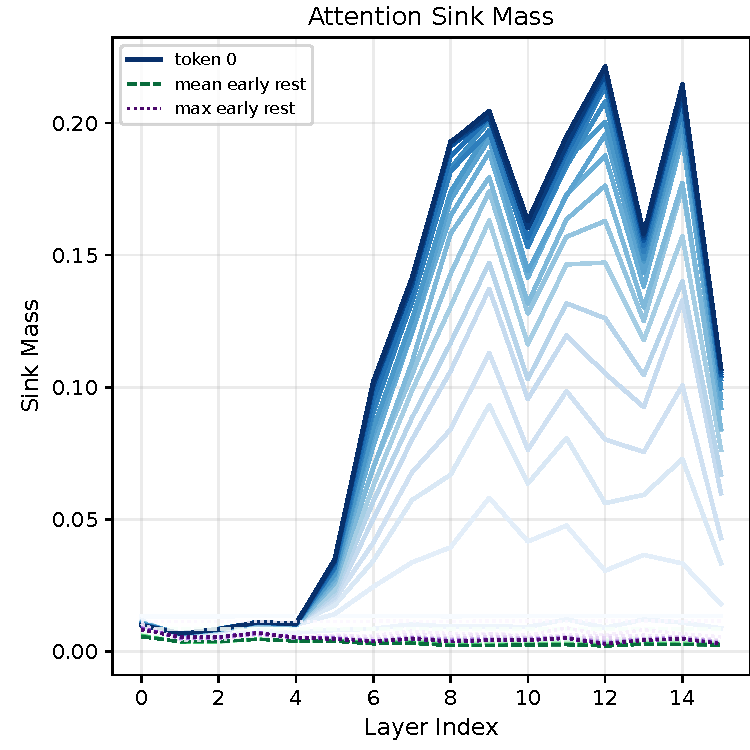
\includegraphics[width=0.23\textwidth]{pics/01B_baseline/AS_mass_compare.pdf}
    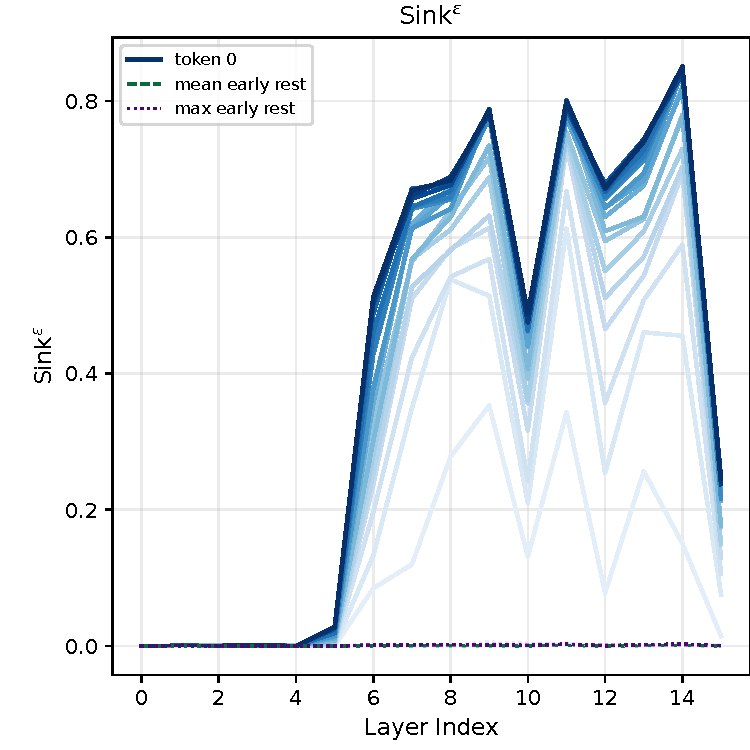
\includegraphics[width=0.23\textwidth]{pics/01B_baseline/AS_eps_compare.pdf}
    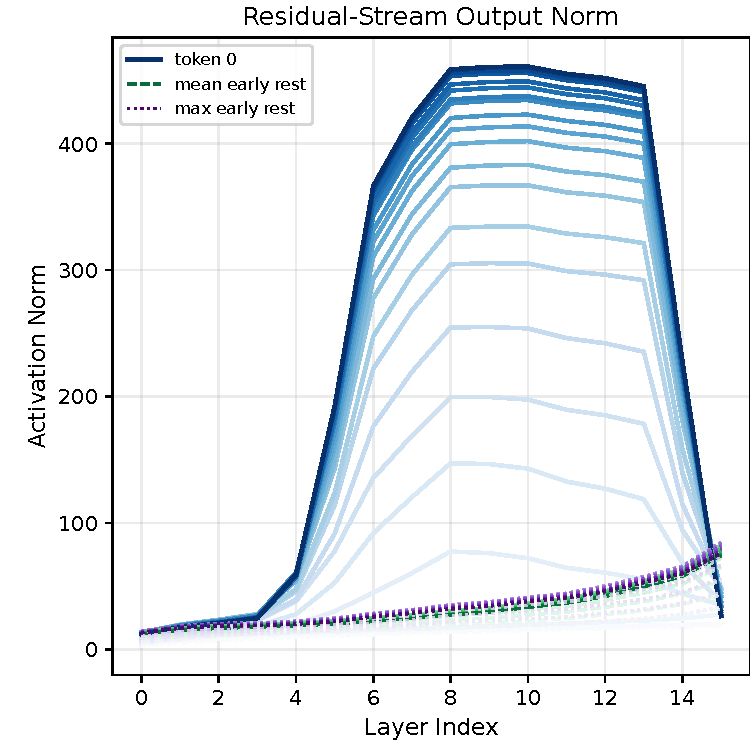
\includegraphics[width=0.23\textwidth]{pics/01B_baseline/MA_x_out_compare.pdf}
    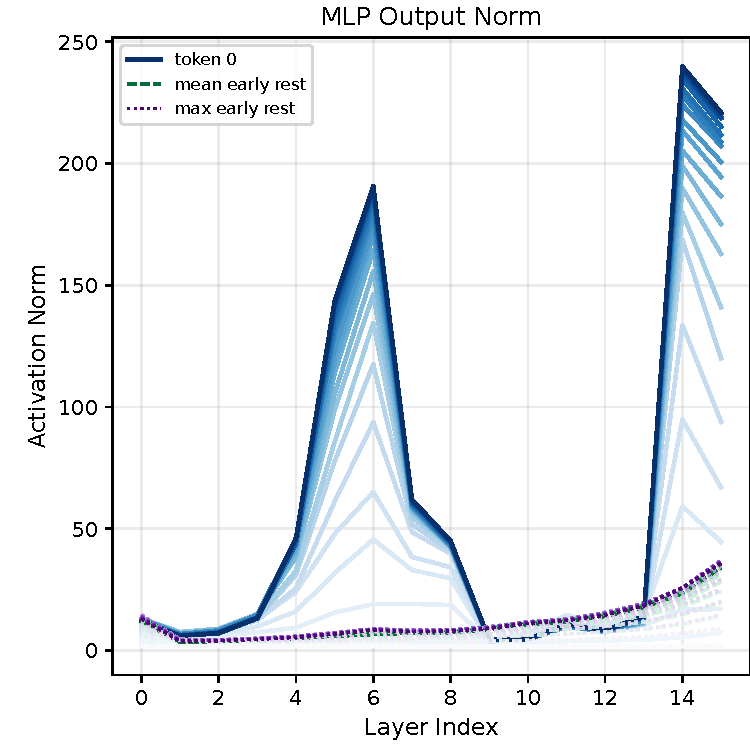
\includegraphics[width=0.23\textwidth]{pics/01B_baseline/MA_mlp_out_compare.pdf}
    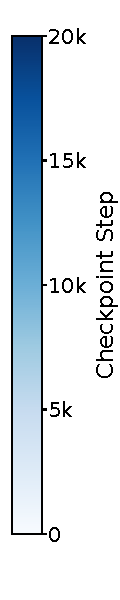
\includegraphics[width=0.046\textwidth]{pics/01B_baseline/extreme_steps.pdf}
    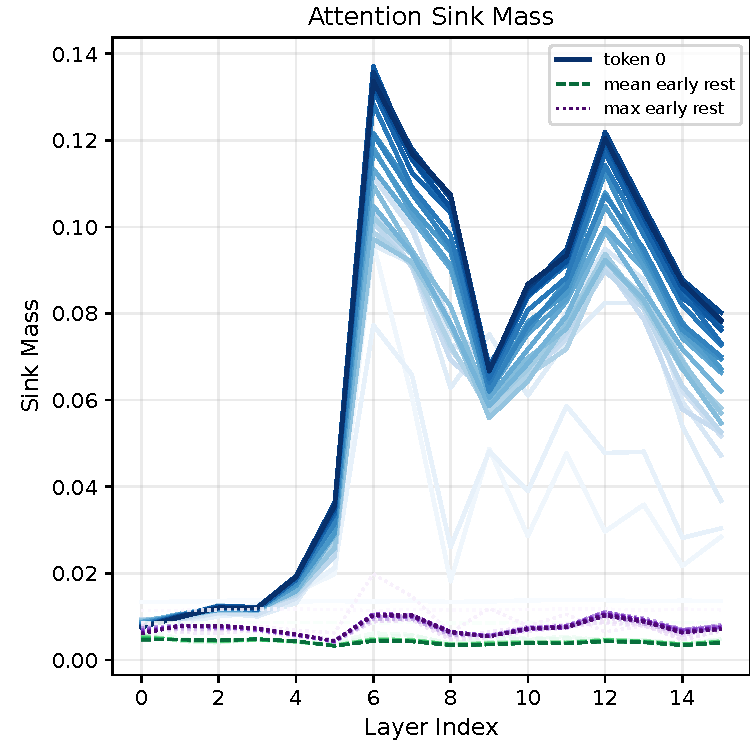
\includegraphics[width=0.23\textwidth]{pics/03B_baseline/AS_mass_compare.pdf}
    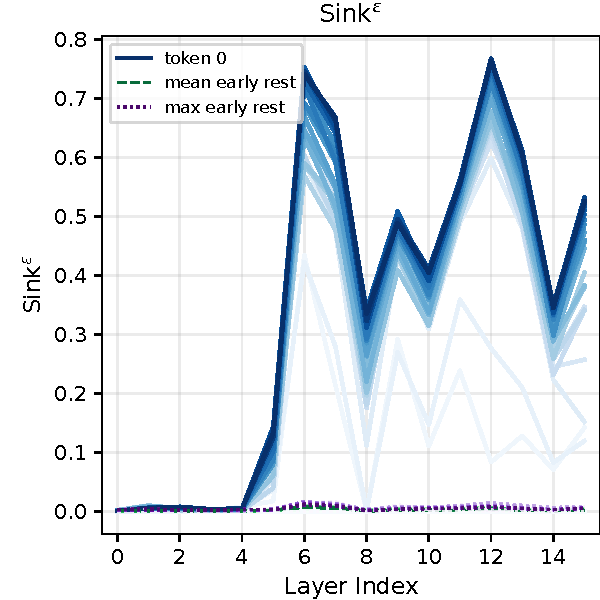
\includegraphics[width=0.23\textwidth]{pics/03B_baseline/AS_eps_compare.pdf}
    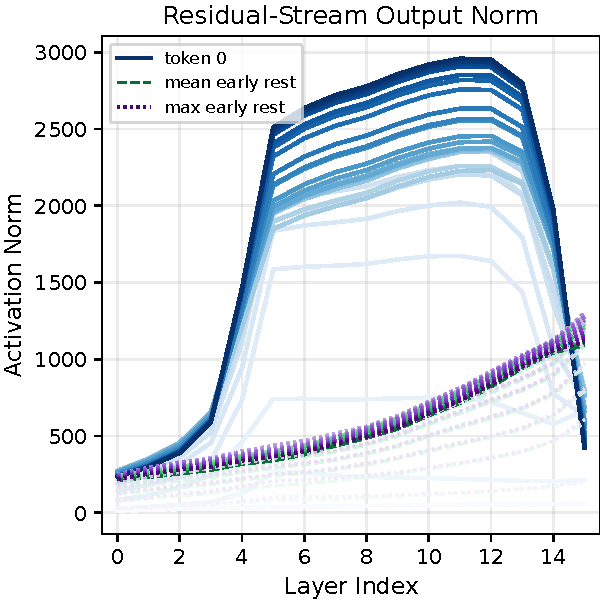
\includegraphics[width=0.23\textwidth]{pics/03B_baseline/MA_x_out_compare.pdf}
    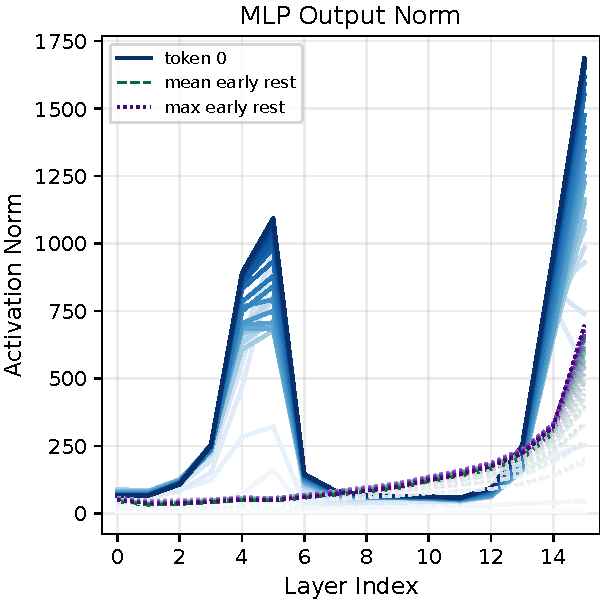
\includegraphics[width=0.23\textwidth]{pics/03B_baseline/MA_mlp_out_compare.pdf}
    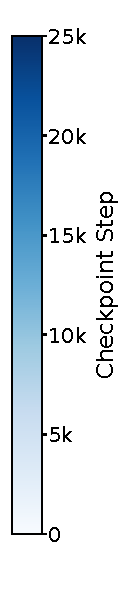
\includegraphics[width=0.046\textwidth]{pics/03B_baseline/extreme_steps.pdf}
    \caption{
    Forward phenomena in baseline models.
    Top row: 0.1B model; bottom row: 0.3B model.
    From left to right: attention sink mass, thresholded sink rate, residual-stream output norm, and MLP output norm.
    The solid blue curve shows token 0, the dashed green curve shows the mean over the rest early tokens, and the dotted purple curve shows their maximum; ``rest early tokens'' refers to positions 1--15.
    The saturation of colors indicates training checkpoints.
    }
    \label{fig:baseline_forward_main}
\end{figure*}

Figure~\ref{fig:baseline_forward_main} summarizes the forward patterns. 
For each plot, the solid blue curve denotes token 0, the dashed green curve denotes the mean over the other early tokens, and the dotted purple curve denotes the maximum over those same early tokens, where ``other early tokens'' refers to token positions 1 to 15. 
In both model sizes, token 0 separates sharply from the other early tokens in the early and middle layers on both Sink Mass $M_s^\ell$ \eqref{eq:sink_mass} and $\mathrm{Sink}_s^{\epsilon}$ \eqref{eq:sink_rate}. 
The activation statistics show a matching pattern. 
On the residual-stream output, token 0 develops a broad elevation across a wide band of middle-to-late layers, whereas the other early tokens increase much more gradually. 
On the MLP output, the distinction is even more localized: token 0 exhibits pronounced peaks at a small number of layers, indicating that the most extreme amplification is produced at specific MLP blocks rather than uniformly across the network.
These forward results show that AS and MA already co-occur clearly in small pretrained pre-norm Transformers.

We now turn to the backward pass and collect the gradients of $q_t$, $k_t$, and $v_t$ in attention blocks for every token position $t$.
For each pathway, we first aggregate gradients over the full batch exactly as in one optimization step, and then take the $l_2$ norm for each token.
This makes the resulting token-wise gradient curves directly comparable to the effective training signal seen by the optimizer.
The statistics are averaged over layers.

\begin{figure*}[tb]
    \centering
    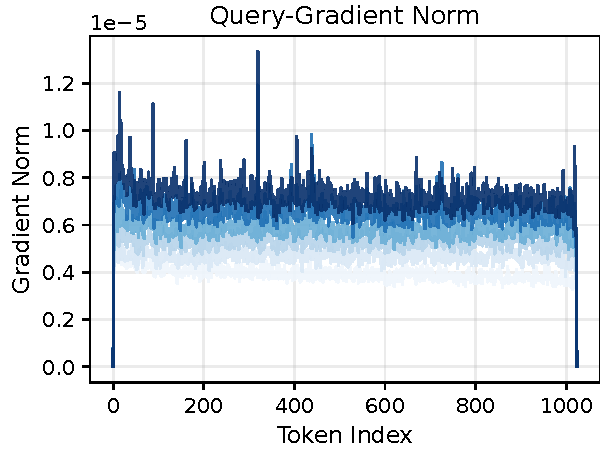
\includegraphics[width=0.3\textwidth]{pics/01B_baseline/LINE_Dq_over_tokens.pdf}
    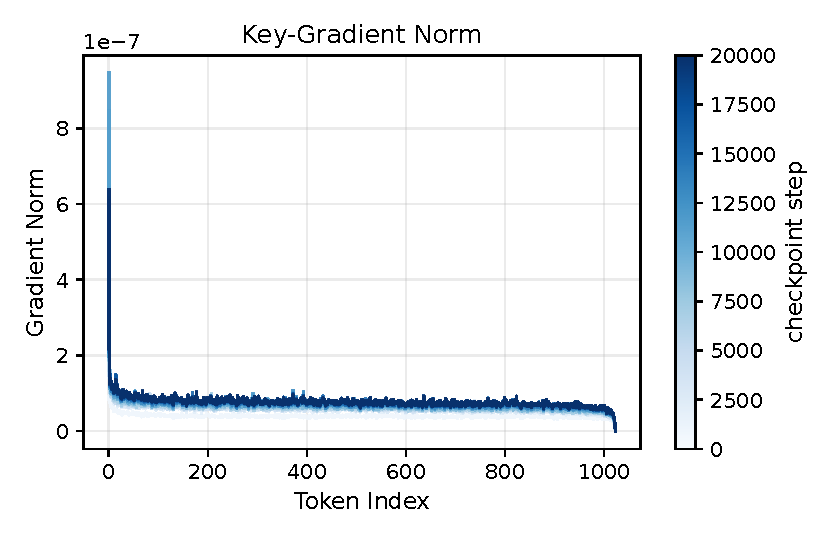
\includegraphics[width=0.3\textwidth]{pics/01B_baseline/LINE_Dk_over_tokens.pdf}
    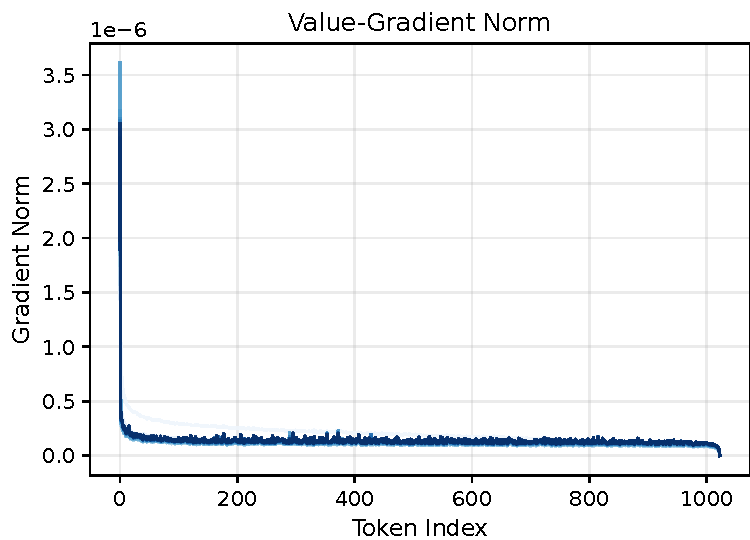
\includegraphics[width=0.3\textwidth]{pics/01B_baseline/LINE_Dv_over_tokens.pdf}
    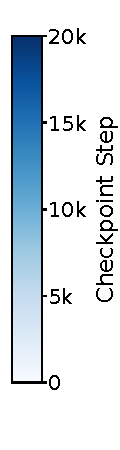
\includegraphics[width=0.06\textwidth]{pics/01B_baseline/line_steps.pdf}
    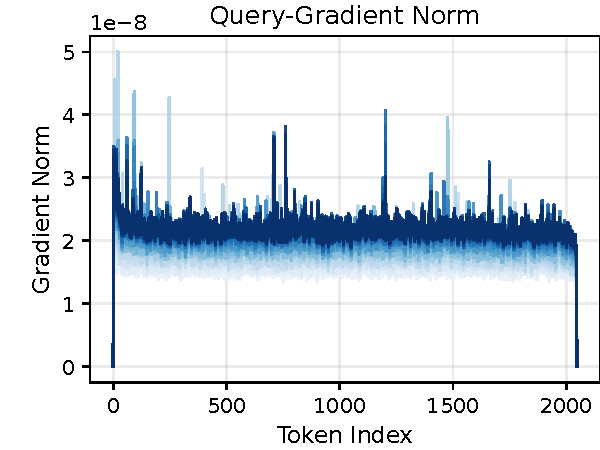
\includegraphics[width=0.3\textwidth]{pics/03B_baseline/LINE_Dq_over_tokens.pdf}
    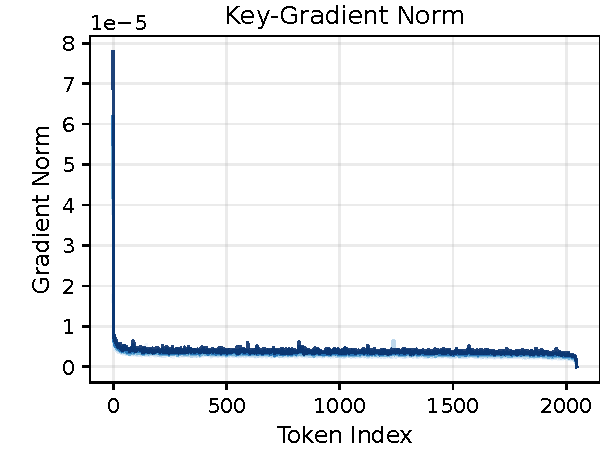
\includegraphics[width=0.3\textwidth]{pics/03B_baseline/LINE_Dk_over_tokens.pdf}
    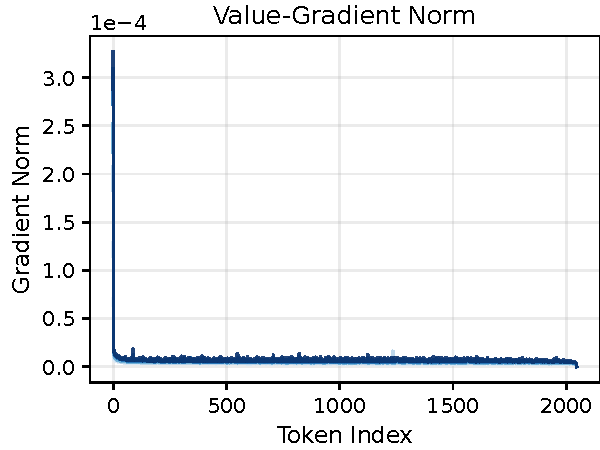
\includegraphics[width=0.3\textwidth]{pics/03B_baseline/LINE_Dv_over_tokens.pdf}
    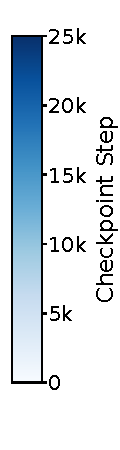
\includegraphics[width=0.06\textwidth]{pics/03B_baseline/line_steps.pdf}
    \caption{
    Token-wise gradient norms of QKV across training checkpoints.
    Top row: 0.1B model; bottom row: 0.3B model.
    From left to right: query gradient norm, key gradient norm, and value gradient norm as functions of token position mean over layers.
    The saturation of colors indicates training checkpoints.
    }
    \label{fig:qkv_grads_over_tokens}
\end{figure*}

Figure~\ref{fig:qkv_grads_over_tokens} shows a clear and highly structured asymmetry.
On the key and value pathways, the gradient norm exhibits a pronounced spike at token 0 across checkpoints, after which it drops rapidly and remains relatively flat over most of the sequence.
This indicates that the dominant backward concentration is not a generic preference for early positions, but a highly localized effect centered on the initial token.
Moreover, the value-side spike is substantially larger than the key-side one, suggesting that the strongest gradient concentration is carried by the value path.

The query pathway looks qualitatively different.
Its token-wise gradient profile is comparatively flat across most positions, and token 0 does not show the same privileged status.
In fact, the query gradient at token 0 is exactly zero under causal mask.
Thus, unlike the key and value pathways, the query pathway does not admit a sink-like gradient concentration at the initial position.
Another consistent feature is that the gradient norms decay to nearly zero at the final token position.

Taken together, these observations establish the central empirical fact of this section:
in pretrained baseline models, the sink token is not only a forward attention sink, but also a backward gradient sink.
More specifically, the gradient sink is strongest on the value path, weaker but still visible on the key path, and absent on the query path.

\subsection{Theoretical results}
\label{subsec:theory_as_to_gs}

We next show that the AS$\Rightarrow$GS link is not just an empirical regularity.
Under causal mask, the value pathway admits an exact aggregation identity, which makes the sink token a backward collector of gradients.
This subsection focuses exclusively on the most central theoretical framework. Supplementary theoretical results and complete proofs are provided in Appendix~\ref{app:proofs}.

Let $g_t := \nabla_{y_t}\mathcal{L} = W_O^\top \nabla_{o_t}\mathcal{L}$ denote the upstream gradient. Recall that $M_s$ and $S_s$~\eqref{eq:sink_mass} denote the sink-column mass and its second moment, respectively. Then by direct computation we have the following formula for exact V-side gradients
\begin{equation}
\label{eq:v_exact_main}
\nabla_{v_s}\mathcal{L}
=
\sum_{t=1}^{T} a_{ts} g_t .
\end{equation}
This identity already exposes the mechanism: the gradient on $v_s$ is an attention-weighted sum of all upstream gradients whose outputs read value from token $s$.. If many later tokens attend to token $s$, then many later gradients also pass through $v_s$. A convenient quantitative version follows from a mean-plus-noise decomposition $g_t = \mu + \varepsilon_t$ for stochastic gradients \citep{mandt2017sgd, mccandlish2018noise}.

\begin{theorem}[V-side gradient control by sink statistics]
\label{thm:v_second_moment_main}
Assume $g_t = \mu + \varepsilon_t$, where $\mathbb{E}[\varepsilon_t]=0$, $\mathrm{Tr}(\mathrm{Cov}(\varepsilon_t)) \le \sigma^2$ for all $t$, and
\[
\big|\mathrm{Tr}(\mathrm{Cov}(\varepsilon_t,\varepsilon_{t'}))\big| \le \rho
\qquad \text{for all } t \ne t'.
\]
Then
\begin{equation}
\label{eq:v_second_moment_main}
\mathbb{E}\big[\|\nabla_{v_s}\mathcal{L}\|_2^2\big]
=
M_s^2\|\mu\|_2^2
+
\sum_{t=1}^{T} a_{ts}^2 \, \mathrm{Tr}(\mathrm{Cov}(\varepsilon_t))
+
\sum_{\substack{t,t'=1 \\ t\ne t'}}^{T} a_{ts} a_{t's} \, \mathrm{Tr}(\mathrm{Cov}(\varepsilon_t,\varepsilon_{t'})).
\end{equation}
In particular,
\begin{equation}
\label{eq:v_second_moment_bound_main}
M_s^2\|\mu\|_2^2
\le
\mathbb{E}\big[\|\nabla_{v_s}\mathcal{L}\|_2^2\big]
\le
M_s^2\|\mu\|_2^2 + \sigma^2 S_s + \rho(M_s^2 - S_s).
\end{equation}
Hence stronger sink columns imply systematically larger value-path gradient concentration.
\end{theorem}

Theorem~\ref{thm:v_second_moment_main} makes AS$\Rightarrow$GS on the value path the central inevitability statement of the paper. We then clarify why value-side interventions should matter most. The same derivation yields exact query/key-path gradients
\begin{equation}
\label{eq:qk_exact_main}
\nabla_{q_s}\mathcal{L}
=
\sum_{j\le s} a_{sj} \beta_{sj} \frac{k_j}{\sqrt d},
\quad
\nabla_{k_s}\mathcal{L}
=
\sum_{t=1}^{T} a_{ts} \beta_{ts} \frac{q_t}{\sqrt d},
\quad
\beta_{ts} := \langle g_t, v_s - y_t \rangle,
\end{equation}
The crucial asymmetry is that K-side gradients aggregate column-wise just as V-side ones, while Q-side gradients are row-local.
For the initial token under causal mask, the attention row contains only self-attention, which gives $\nabla_{q_0}\mathcal{L} = 0$. This matches our measurements: the sink token shows strong value/key gradient concentration but no special Q-side advantage.

\section{Gradient Reshaping by Massive Activations}
\label{sec:pressure_reshape}
Section~\ref{sec:as_to_gs} established that attention sinks are also gradient sinks, with the strongest concentration appearing on the value path.  
We now examine how this sink-centered gradient pressure is reshaped inside pre-norm residual blocks.  
What we show in this section is an empirical three-stage pattern: the sink token experiences strong branch-local gradient amplification (\emph{Bloat}), disproportionately strong normalization-aligned attenuation (\emph{Compress}), and yet only moderate net gradient change across the residual transition (\emph{Change}).  

We begin with the attention branch.
For each layer of a checkpoint, we compare the activation norms of the branch input, $\|h_{\mathrm{in}}^\ell\|$, against one of the three ratios defined in \eqref{eq:ratios_attn}:
\[
\mathrm{Bloat}^{\mathrm{attn},\ell},\quad
\mathrm{Compress}^{\mathrm{attn},\ell},\quad
\mathrm{Change}^{\mathrm{attn},\ell}.
\]
The scatter plots are colored by token group: token 0, token 1, tokens 2--3, tokens 4--7, and the remaining early tokens (8--15).
This visualization makes it possible to see simultaneously \emph{where} large gradient pressure appears, \emph{where} strong attenuation happens, and whether the final residual-stream gradient ratio remains stable.

\begin{figure*}[t]
    \centering
    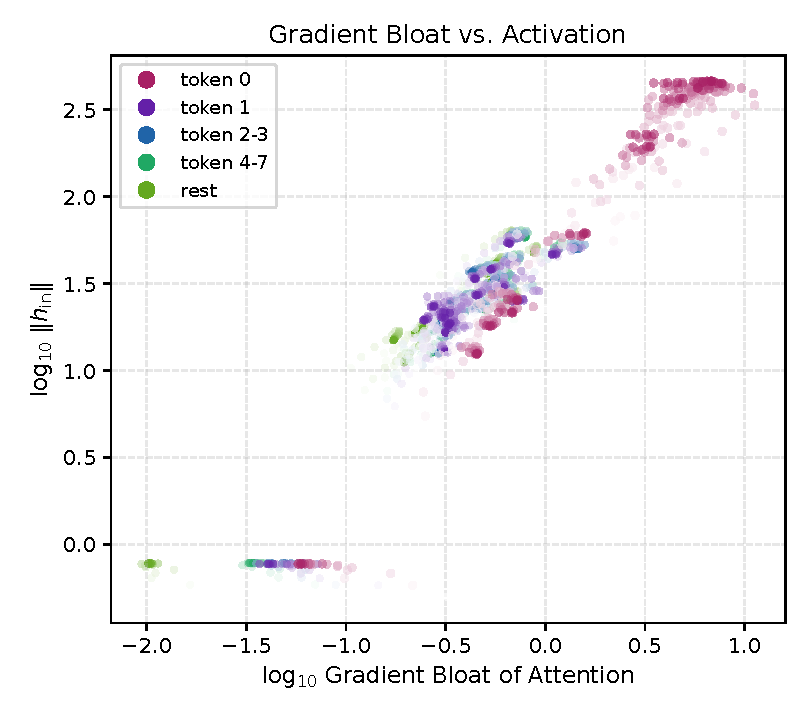
\includegraphics[width=0.3\linewidth]{pics/01B_baseline/Ea3_Bloat.pdf}
    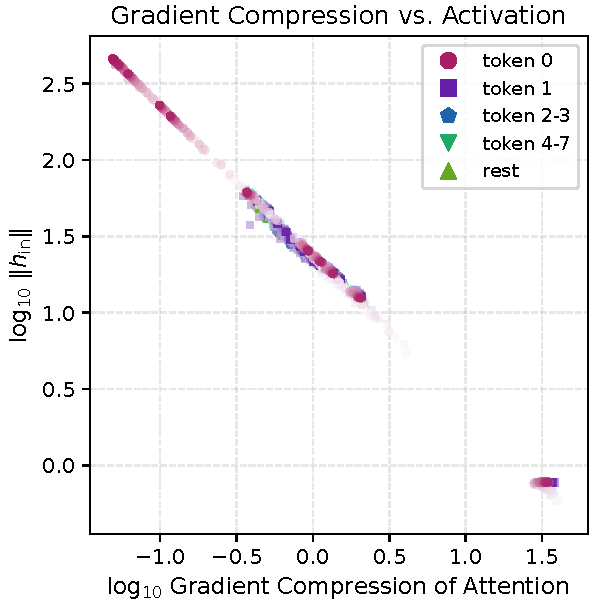
\includegraphics[width=0.3\linewidth]{pics/01B_baseline/Ea1_compress.pdf}
    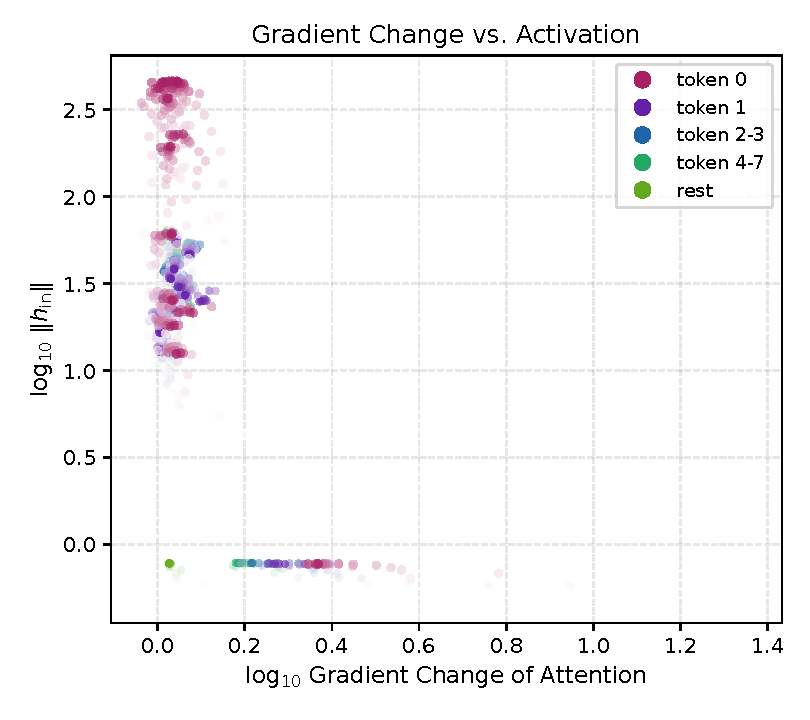
\includegraphics[width=0.3\linewidth]{pics/01B_baseline/Ea4_Change.pdf}
    \includegraphics[width=0.06\linewidth]{pics/01B_baseline/scatter_group_steps.pdf}
    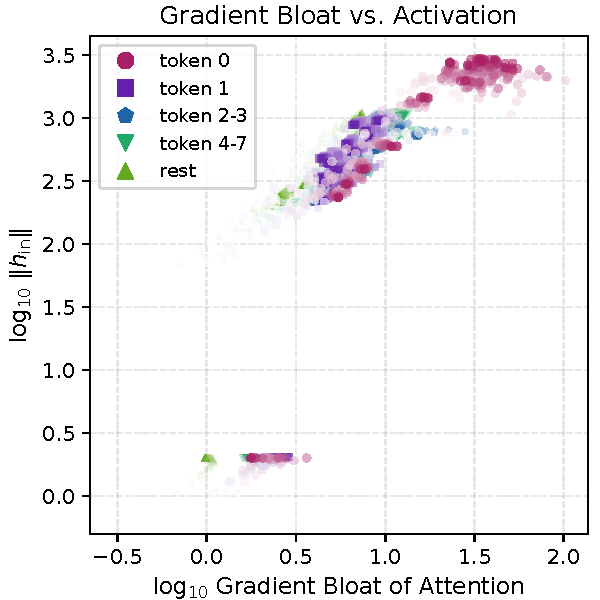
\includegraphics[width=0.3\linewidth]{pics/03B_baseline/Ea3_Bloat.pdf}
    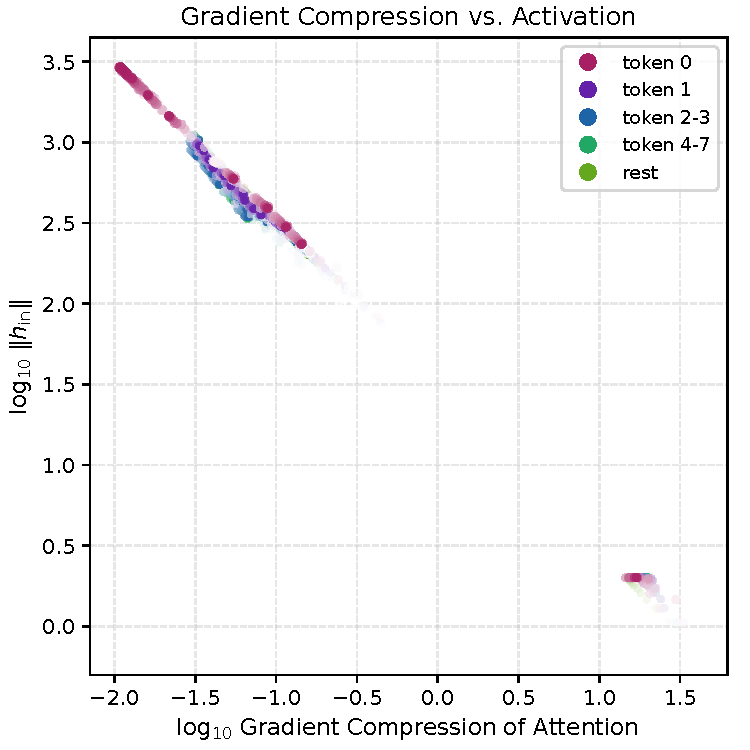
\includegraphics[width=0.3\linewidth]{pics/03B_baseline/Ea1_compress.pdf}
    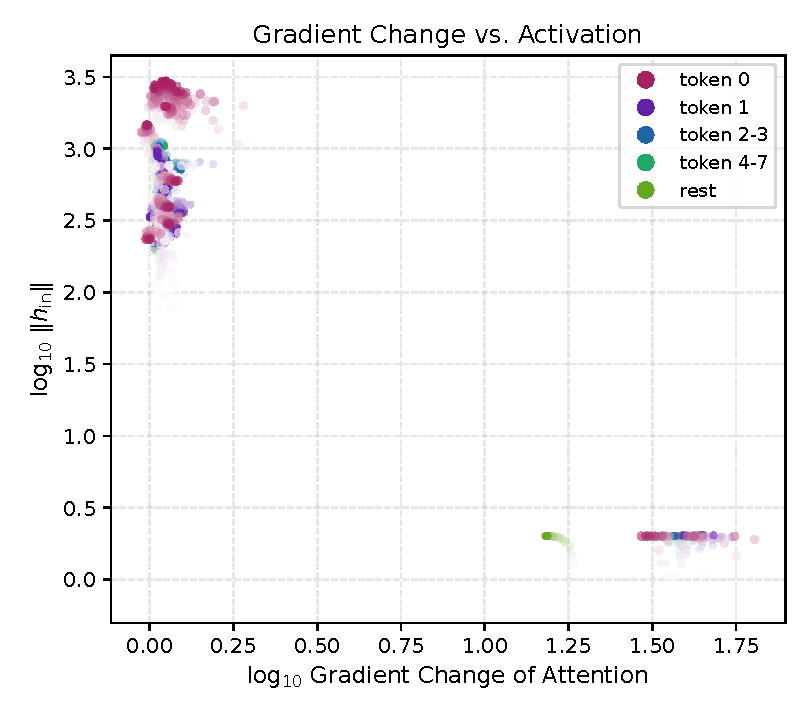
\includegraphics[width=0.3\linewidth]{pics/03B_baseline/Ea4_Change.pdf}
    \includegraphics[width=0.06\linewidth]{pics/03B_baseline/scatter_group_steps.pdf}
    \caption{
    Attention-side scatter plots relating gradient reshaping to activation magnitude. Top row: 0.1B model; bottom row: 0.3B model.
    From left to right: $\log_{10}\mathrm{Bloat}^{\mathrm{attn}}$ vs.\ $\log_{10}\|h_{\mathrm{in}}\|$, 
    $\log_{10}\mathrm{Compress}^{\mathrm{attn}}$ vs.\ $\log_{10}\|h_{\mathrm{in}}\|$, and
    $\log_{10}\mathrm{Change}^{\mathrm{attn}}$ vs.\ $\log_{10}\|h_{\mathrm{in}}\|$.
    Each point is colored by token group (token 0, token 1, tokens 2--3, tokens 4--7, and the rest).
    The left panel shows that large activation points, especially those from token 0, are also the points with the largest branch-local gradient bloat.
    The middle panel shows that activation magnitude is tightly aligned with RMSNorm-mediated attenuation.
    The right panel shows that despite large local reshaping, most high-activation points remain close to $\log_{10}1=0$, i.e., near unit net gradient change across the residual transition.
    }
    \label{fig:attn_scatter_main}
\end{figure*}

Figure~\ref{fig:attn_scatter_main} shows that these three quantities play sharply different roles.
In the left panel, large activation points concentrate in the high-bloat regime, and this region is dominated by token 0.
This means that the sink token is not merely a place where gradients are large in an absolute sense; it is specifically the place where the attention branch locally amplifies gradient norm most strongly.
By contrast, the remaining tokens mostly populate a much milder regime.
Thus, the backward pressure created by the gradient sink is highly localized rather than uniformly distributed across the sequence.

The middle panel shows an equally striking structure for $\mathrm{Compress}^{\mathrm{attn}}$.
Rather than forming a broad cloud, the points collapse onto an almost one-dimensional trend, indicating that RMSNorm-mediated attenuation is tightly controlled by activation magnitude.
High-activation points lie systematically at the strong-attenuation end of this curve, while low-activation points occupy the weak-attenuation regime.
In other words, once strong branch-local pressure is created, the normalization layer does not attenuate it arbitrarily; the amount of attenuation is strongly aligned with the scale of the token activation itself.
This is exactly the empirical pattern expected if large activations act as an effective gradient-compression channel in pre-norm computation.

The right panel explains why this alignment matters.
Although $\mathrm{Bloat}^{\mathrm{attn}}$ can become very large on high-activation sink-centered points, the corresponding $\mathrm{Change}^{\mathrm{attn}}$ values remain concentrated near $\log_{10}1 = 0$, especially in the high-activation regime.
That is, the net gradient ratio across the residual transition stays close to one even when the branch internally exhibits strong amplification and strong compression.
This observation is important because it distinguishes \emph{local gradient pressure} from \emph{global gradient instability}.
If large bloat directly translated into equally large net residual-stream gradients, one would expect severe cross-layer gradient explosion.
Instead, what we observe is a reshaping pattern: large branch-local pressure is largely compensated before it re-enters the residual stream.

This near-unit net change is also consistent with the broader literature on trainable deep residual architectures.
A major reason residual networks remain optimizable at depth is that signal propagation stays close to identity in an appropriate sense, rather than drifting into systematic explosion or collapse \citep{he2016deep,xiong2020layernorm,zhang2019fixup,liu2020understanding,bachlechner2021rezero,wang2022deepnet}.
From this perspective, $\mathrm{Change}\approx 1$ is not a cosmetic detail.
It indicates that the sink-centered branch pressure revealed by $\mathrm{Bloat}$ is not simply passed upstream unchecked; instead, it is reshaped into a regime compatible with stable residual propagation.
This is precisely why the distinction between \emph{Bloat}, \emph{Compress}, and \emph{Change} is necessary: only the first exposes where pressure is created, only the second shows how it is attenuated, and only the third reveals whether the final gradient signal remains in a stable range.

Taken together, Figure~\ref{fig:attn_scatter_main} suggests the following picture.
The sink token experiences unusually strong branch-local gradient amplification in attention; high activation magnitude is tightly aligned with strong normalization-induced attenuation; and after this reshaping, the net gradient ratio across the residual transition remains close to one.
We emphasize again that this section does not yet prove that massive activations are \emph{caused} by gradient sinks.
What it does show is that large activations are systematically aligned with the very locations where sink-centered gradient pressure is strongest and where the strongest attenuation is required.

\subsection{Bridge to the next step}
\label{subsec:reshaping_bridge}

The analysis above establishes a stable empirical pattern, but it still leaves one key question open:
which backward pathway is primarily carrying this mechanism?
The next section addresses this by intervening directly on different gradient paths.
If the picture above is meaningful, then weakening the relevant backward pathway should reduce the need for such strong activation-aligned attenuation.
















We first examine the three backward ratios in the attention branch defined in \eqref{eq:ratios_attn}. 
Figure~\ref{fig:attn_bloat_compress_change} shows a consistent pattern across model sizes and checkpoints.  
On the initial token, \emph{Bloat}$^{\mathrm{attn}}$ is substantially larger than other early tokens.  
This indicates that once backward pressure has concentrated on the sink token, the attention branch further amplifies that pressure locally before it reaches the pre-attention residual representation.
At the same time, the sink token also shows markedly larger \emph{Compress}$^{\mathrm{attn}}$.  
Thus the same token that experiences the strongest local branch pressure is also the one on which the norm layer attenuates gradients the most.  
This pairing is important: it shows that the network is not simply passing sink-centered pressure backward unchanged.  
Instead, the branch first inflates the local gradient norm and the norm layer then suppresses a substantial fraction of that inflated signal.
Most importantly, \emph{Change}$^{\mathrm{attn}}$ is far less extreme than \emph{Bloat}$^{\mathrm{attn}}$.  
In many layers the sink token has very large branch-local amplification while the net residual-stream gradient ratio remains much closer to $1$.  
This is exactly the regime discussed in Section~\ref{subsec:why_change_matters}: large localized pressure is present, but it is not simply converted into equally large net gradient amplification across depth.


\begin{figure*}[t]
    \centering
    \fbox{\parbox{0.96\textwidth}{
    \vspace{1.3cm}
    \centering
    \textbf{Placeholder for attention-branch Bloat/Compress/Change.}\\[0.4em]
    Suggested layout: a $2\times 3$ figure with rows for 0.1B / 0.3B and columns for
    $\mathrm{Bloat}^{\mathrm{attn}}$, $\mathrm{Compress}^{\mathrm{attn}}$, and $\mathrm{Change}^{\mathrm{attn}}$.\\
    Main visual message: token 0 shows much larger Bloat and Compress than other early tokens, while Change stays far closer to $1$.
    \vspace{1.3cm}
    }}
    \caption{Attention-branch gradient reshaping.  The sink token exhibits strong branch-local amplification and strong attenuation, but only moderate net gradient change across the residual transition.}
    \label{fig:attn_bloat_compress_change}
\end{figure*}





\subsection{Why net \textit{Change} near 1 matters}
\label{subsec:why_change_matters}

The quantity
\[
\mathrm{Change}_t
= \frac{\|G(h_t^{\mathrm{in}})\|_2}{\|G(h_t^{\mathrm{out}})\|_2}
\]
measures the net gradient ratio across a residual transition.  
This ratio is important because stable deep optimization generally benefits from approximately scale-preserving signal and gradient propagation: residual identity mappings help forward and backward signals pass directly across depth \citep{he2016identity}, dynamical-isometry analyses emphasize Jacobian singular values concentrated near $1$ \citep{pennington2017resurrecting,schoenholz2017deep}, and several deep-residual / Transformer stabilization methods are explicitly designed to keep residual updates from dominating the skip path \citep{zhang2019fixup,liu2020understanding,bachlechner2021rezero,wang2022deepnet}.  
In the Transformer setting, Pre-LN architectures are also known to have substantially better-behaved gradients than Post-LN ones at initialization \citep{xiong2020layernorm}.

Against this background, observing large \emph{Bloat} alone is not yet enough to interpret the training dynamics.  
If the sink token also had very large \emph{Change}, then the phenomenon could be explained simply as net gradient explosion propagating directly through depth.  
By contrast, if \emph{Bloat} is large while \emph{Change} remains close to $1$, then the picture is qualitatively different: strong local pressure is being created inside the branch, but it is not being transmitted to the residual stream in equally amplified form.  
This makes \emph{Change} the key quantity that separates \emph{localized branch pressure} from \emph{global gradient instability}.

A simple residual identity makes this precise.  
For the attention block,
\[
G(h_t^{\ell})
=
G(h_t^{\ell+\frac12})
+
\bigl(G(h_t^{\ell}) - G(h_t^{\ell+\frac12})\bigr),
\]
and analogously for the MLP block.  
Thus, \emph{Change} measures the norm ratio after the identity path and the branch contribution have been recombined.  
If this ratio stays near $1$, the residual stream continues to propagate gradients at roughly the same scale even though the branch itself may have produced a large token-specific perturbation.  
For our mechanism, this distinction is essential: the sink token is special not because the entire network becomes globally unstable there, but because large local pressure is selectively generated and then selectively attenuated.

\subsection{MLP branch: compression remains aligned with large activations}
\label{subsec:mlp_bloat_compress_change}

We next examine the same three ratios in the MLP branch.
Although the MLP branch is not where AS is created, it is where the most visible massive activations are formed in Figure~\ref{fig:baseline_forward_main}.  
This makes it the natural place to ask whether large activation magnitude is aligned with strong gradient attenuation.

\begin{figure*}[t]
    \centering
    \fbox{\parbox{0.96\textwidth}{
    \vspace{1.3cm}
    \centering
    \textbf{Placeholder for MLP-branch Bloat/Compress/Change.}\\[0.4em]
    Suggested layout: a $2\times 3$ figure with rows for 0.1B / 0.3B and columns for
    $\mathrm{Bloat}^{\mathrm{mlp}}$, $\mathrm{Compress}^{\mathrm{mlp}}$, and $\mathrm{Change}^{\mathrm{mlp}}$.\\
    Main visual message: sink-centered pressure continues into the MLP branch, and strong compression coincides with layers where token-0 MLP activations are large.
    \vspace{1.3cm}
    }}
    \caption{MLP-branch gradient reshaping.  The sink token again shows strong compression, now aligned with the layers where MLP-output norms are unusually large.}
    \label{fig:mlp_bloat_compress_change}
\end{figure*}

The MLP-side picture is different in detail but similar in logic.  
The sink token again exhibits distinctive branch-local reshaping, and the strongest \emph{Compress}$^{\mathrm{mlp}}$ values occur precisely in the layers where Figure~\ref{fig:baseline_forward_main} showed the largest token-0 MLP-output norms.  
This alignment is the main reason we introduce MA in this section at all: not as a proved consequence of GS, but as a forward signature that systematically co-locates with strong gradient attenuation.

Crucially, the same caveat remains in force.  
These results do \emph{not} by themselves show that GS causally induces MA.  
They show something weaker but still highly informative: massive activations are not arbitrary forward anomalies.  
They appear at precisely the token-layer locations where the network is also attenuating unusually strong branch-specific backward signals.

\subsection{Activation magnitude and compression are tightly aligned}
\label{subsec:act_compress_alignment}

To make this alignment explicit, we directly compare activation magnitude with the corresponding compression statistics.

\begin{figure}[t]
    \centering
    \fbox{\parbox{0.92\linewidth}{
    \vspace{1.2cm}
    \centering
    \textbf{Placeholder for activation--compression alignment.}\\[0.4em]
    Suggested content: scatter plot or paired curves relating token/layer activation norm to
    $\mathrm{Compress}^{\mathrm{attn}}$ or $\mathrm{Compress}^{\mathrm{mlp}}$.\\
    Main visual message: large activation norm is strongly associated with strong compression on the same token and layer.
    \vspace{1.2cm}
    }}
    \caption{Activation magnitude aligns with normalization-induced compression.  High-norm sink-token activations are systematically associated with stronger attenuation of backward signals.}
    \label{fig:act_compress_alignment}
\end{figure}

Figure~\ref{fig:act_compress_alignment} shows that high activation magnitude and strong compression are tightly aligned across token-layer instances.  
This observation is consistent with the Appendix result that the RMSNorm Jacobian scales inversely with the input RMS magnitude: larger incoming residual norm implies a smaller local backward operator norm, all else equal.  
Empirically, this is exactly the pattern we observe on sink tokens.  
Where activation magnitude becomes unusually large, backward attenuation also becomes unusually strong.

This alignment is the main bridge from the gradient language of this paper to the activation language of the MA literature.  
Section~\ref{sec:as_to_gs} showed that sink tokens collect gradient pressure.  
The present section shows that inside pre-norm residual blocks, such pressure is first amplified, then strongly attenuated at precisely those token-layer locations where activations are large, and finally leaves only a much milder net gradient change across the residual stream.

\subsection{Takeaway}
\label{subsec:pressure_reshape_takeaway}

The main message of this section is therefore a \emph{reshaping} statement rather than a causal one.  
Sink-centered gradients are not merely large; they are selectively processed by pre-norm computation.  
The sink token exhibits substantial branch-local amplification (Bloat), disproportionately strong normalization-induced attenuation (Compress), and only moderate net gradient change (Change).  
Because the strongest compression aligns with the largest activation magnitudes, these results are consistent with viewing massive activations as a forward signature of the network's attenuation of localized gradient pressure.

This still does not identify which backward pathway is most responsible for the effect.  
That is the purpose of the next section, where we intervene directly on different gradient paths to determine which one actually carries the mechanism.



































\begin{figure}[htbp]
    \centering
    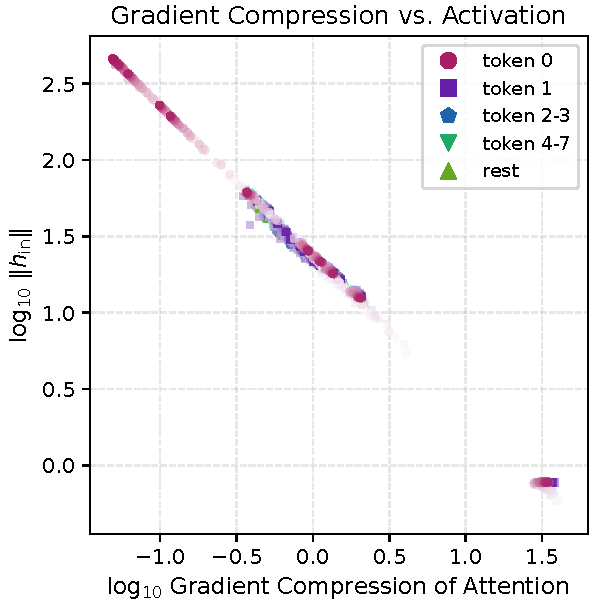
\includegraphics[width=0.3\linewidth]{pics/01B_baseline/Ea1_compress.pdf}
    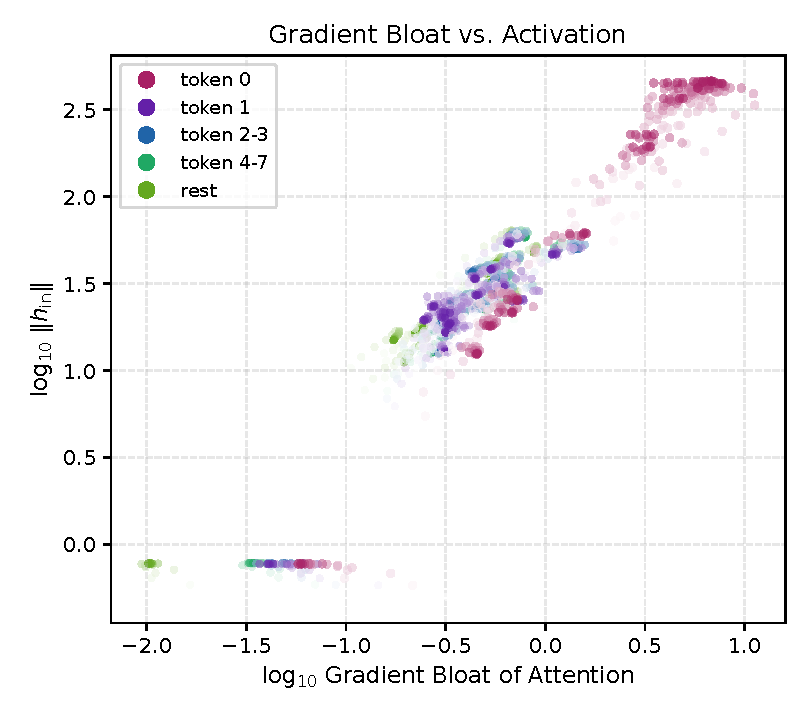
\includegraphics[width=0.3\linewidth]{pics/01B_baseline/Ea3_Bloat.pdf}
    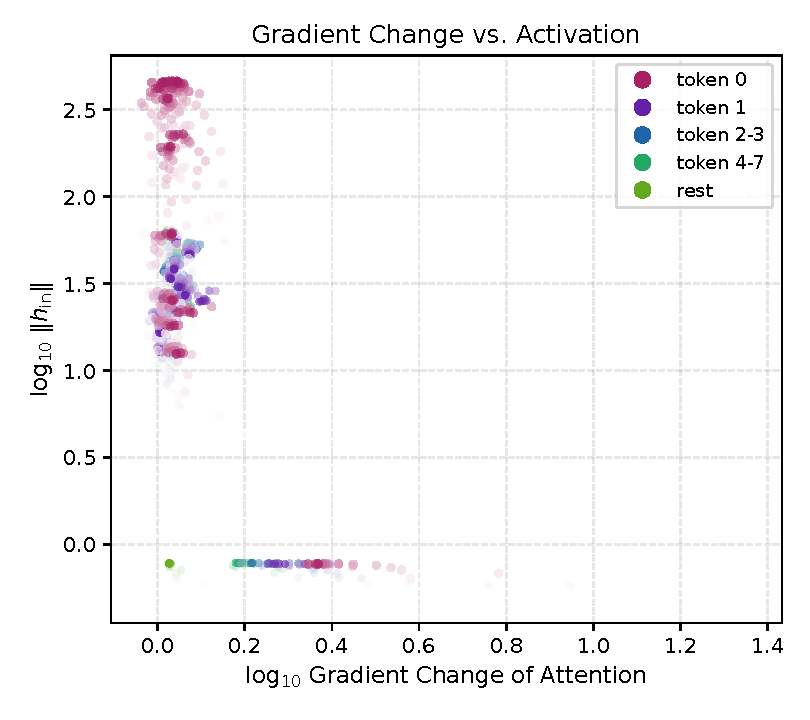
\includegraphics[width=0.3\linewidth]{pics/01B_baseline/Ea4_Change.pdf}
    \includegraphics[width=0.06\linewidth]{pics/01B_baseline/scatter_group_steps.pdf}
    \caption{Main results with a shared colorbar.}
\end{figure}
\begin{figure}[htbp]
    \centering
    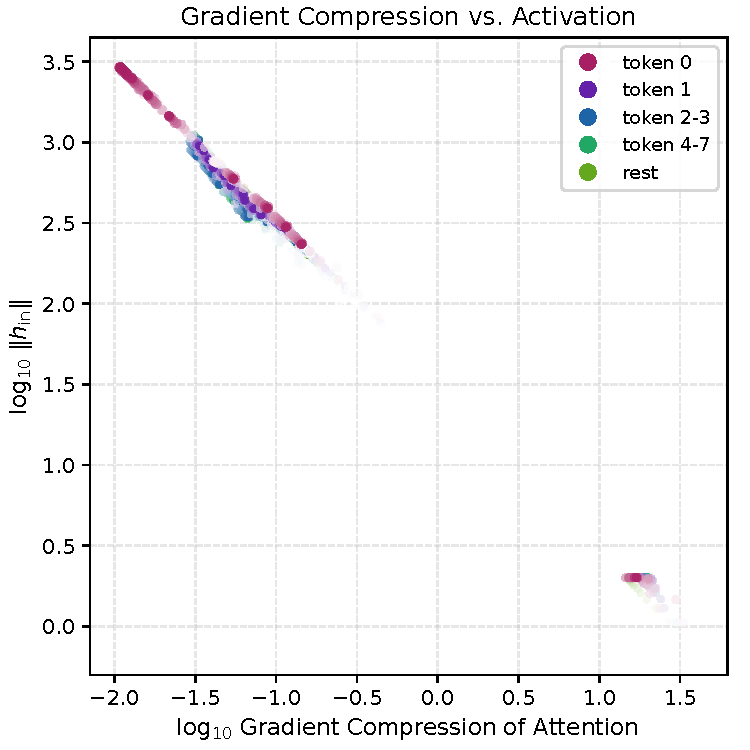
\includegraphics[width=0.3\linewidth]{pics/03B_baseline/Ea1_compress.pdf}
    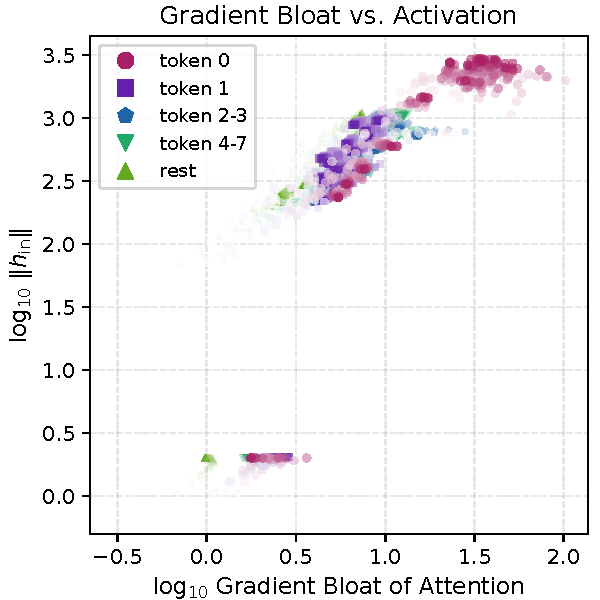
\includegraphics[width=0.3\linewidth]{pics/03B_baseline/Ea3_Bloat.pdf}
    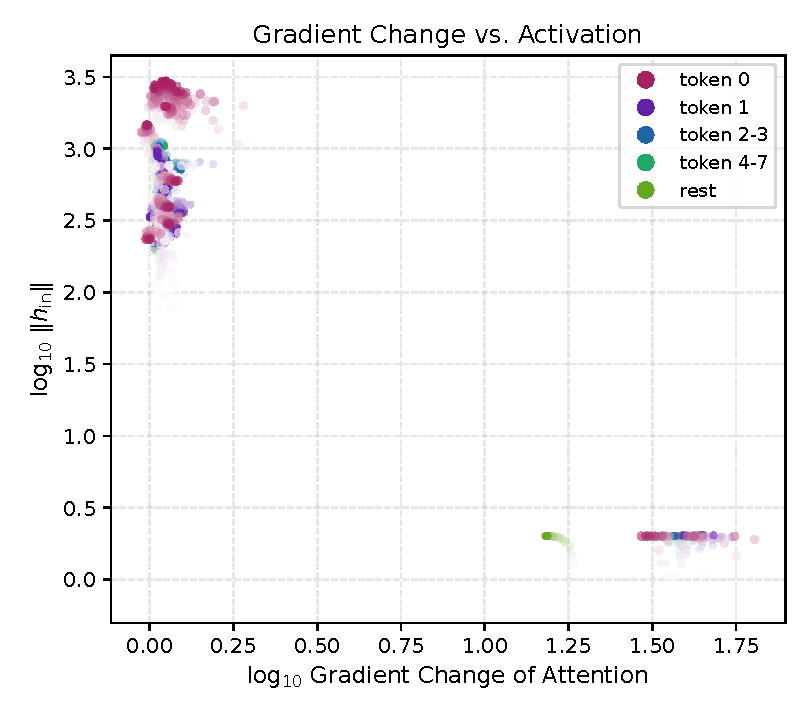
\includegraphics[width=0.3\linewidth]{pics/03B_baseline/Ea4_Change.pdf}
    \includegraphics[width=0.06\linewidth]{pics/03B_baseline/scatter_group_steps.pdf}
    \caption{Main results with a shared colorbar.}
\end{figure}


\begin{figure}[htbp]
    \centering
    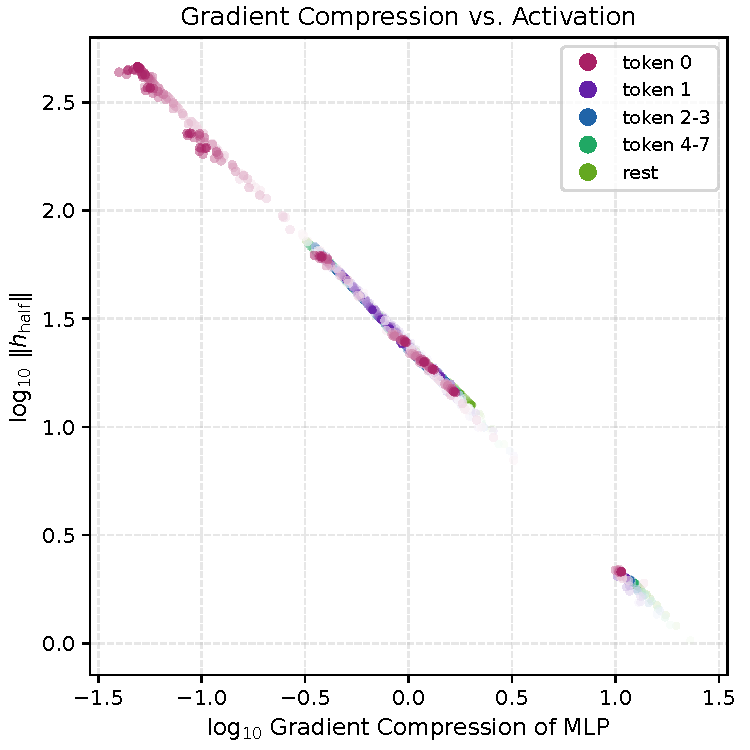
\includegraphics[width=0.3\linewidth]{pics/01B_baseline/Em1_compress.pdf}
    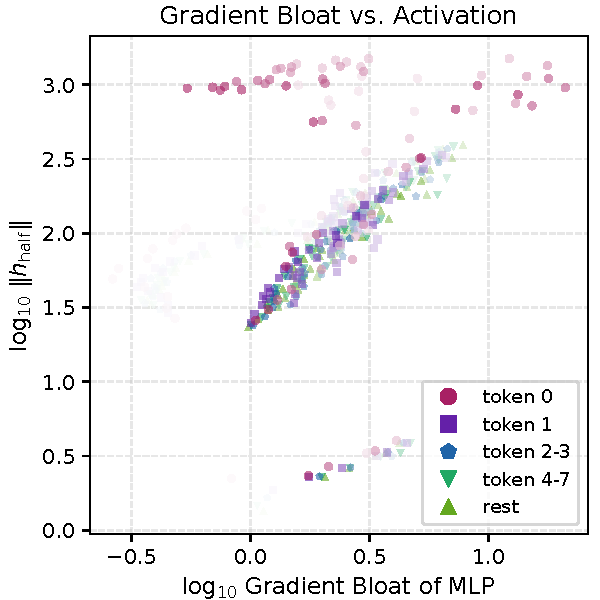
\includegraphics[width=0.3\linewidth]{pics/01B_baseline/Em3_Bloat.pdf}
    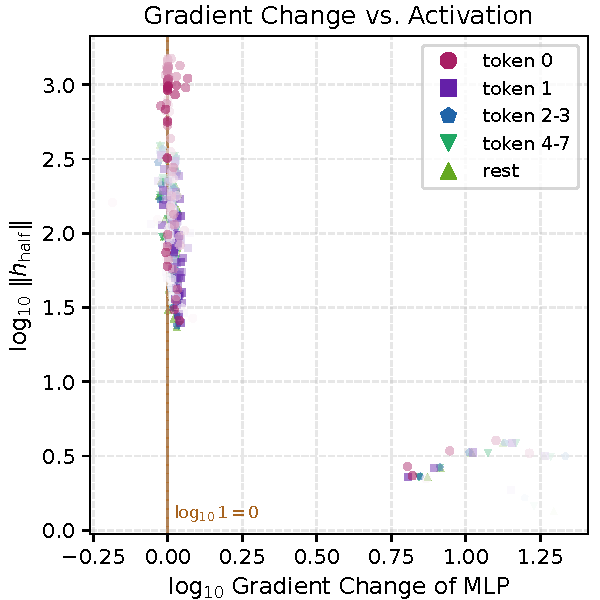
\includegraphics[width=0.3\linewidth]{pics/01B_baseline/Em4_Change.pdf}
    \includegraphics[width=0.06\linewidth]{pics/01B_baseline/scatter_group_steps.pdf}
    \caption{Main results with a shared colorbar.}
\end{figure}
\begin{figure}[htbp]
    \centering
    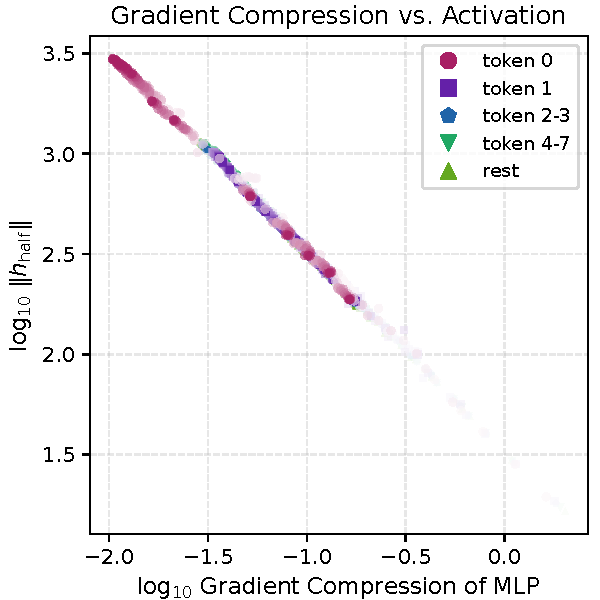
\includegraphics[width=0.3\linewidth]{pics/03B_baseline/Em1_compress.pdf}
    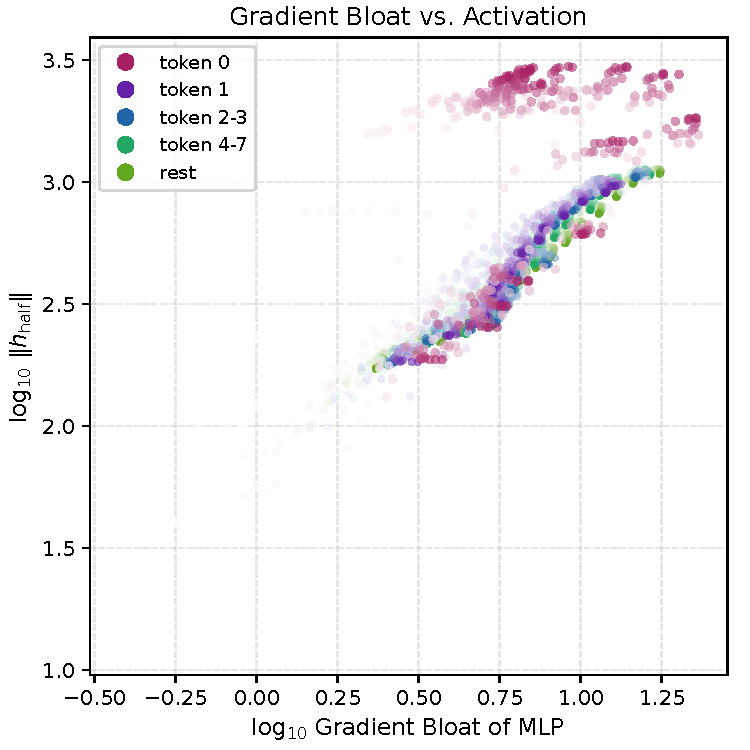
\includegraphics[width=0.3\linewidth]{pics/03B_baseline/Em3_Bloat.pdf}
    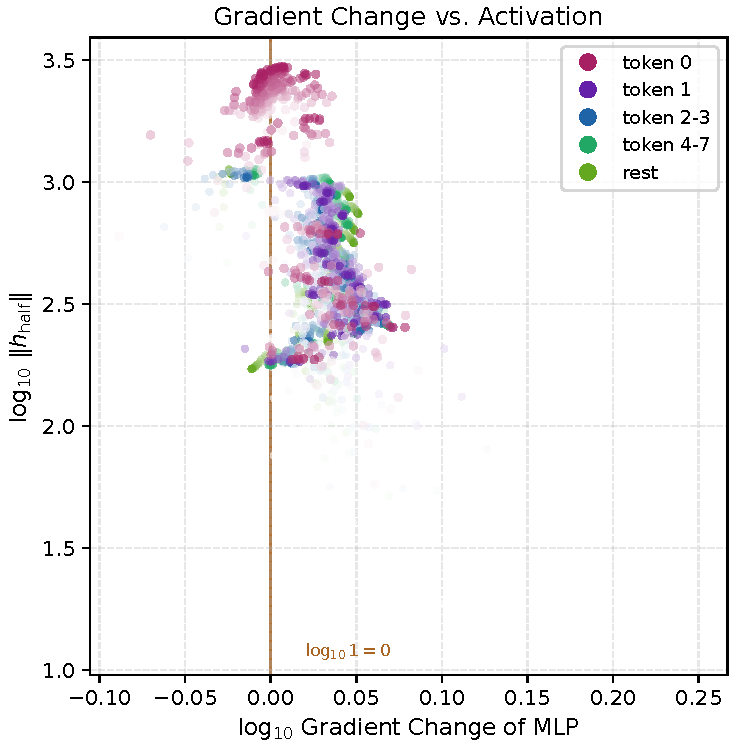
\includegraphics[width=0.3\linewidth]{pics/03B_baseline/Em4_Change.pdf}
    \includegraphics[width=0.06\linewidth]{pics/03B_baseline/scatter_group_steps.pdf}
    \caption{Main results with a shared colorbar.}
\end{figure}


\begin{figure}[htbp]
    \centering
    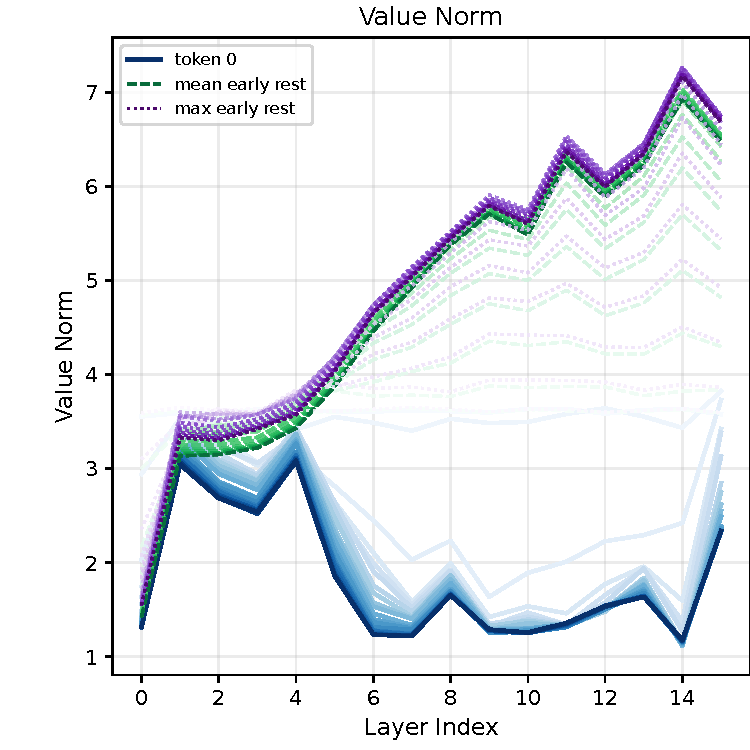
\includegraphics[width=0.3\linewidth]{pics/01B_baseline/V_norm_compare.pdf}
    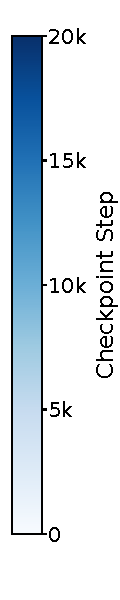
\includegraphics[width=0.06\linewidth]{pics/01B_baseline/extreme_steps.pdf}
    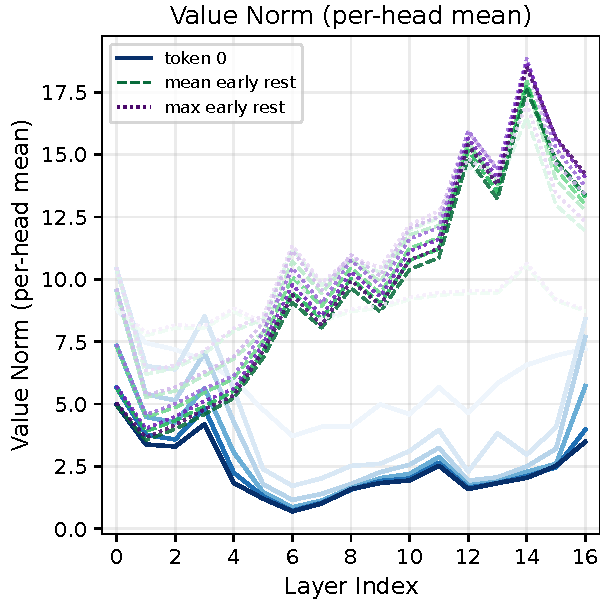
\includegraphics[width=0.3\linewidth]{pics/03B_baseline/V_norm_compare.pdf}
    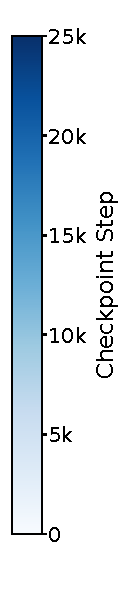
\includegraphics[width=0.06\linewidth]{pics/03B_baseline/extreme_steps.pdf}
    \caption{Main results with a shared colorbar.}
\end{figure}




\subsection{RMSNorm makes large activations a gradient compressor}
For RMSNorm \citep{zhang2019rmsnorm},
\[
\mathrm{RMSNorm}(x)=\gamma \odot \frac{x}{\rms(x)},\qquad \rms(x)=\sqrt{\frac{1}{d}\sum_i x_i^2}.
\]
Its Jacobian obeys a simple operator-norm bound.

\begin{proposition}[RMSNorm compression]
Let $J_{\mathrm{rms}}(x)$ be the Jacobian of RMSNorm. Then
\[
\|J_{\mathrm{rms}}(x)\|_{\mathrm{op}} \le \frac{2\|\gamma\|_\infty}{\rms(x)}.
\]
Consequently,
\[
\|\nabla_x\mathcal{L}\| \lesssim \frac{1}{\rms(x)}\|\nabla_y\mathcal{L}\|.
\]
Increasing the input norm reduces the backpropagated gradient norm.
\end{proposition}

This is the bridge from GS to MA. In a pre-norm Transformer, large token activation is not primarily useful because it changes the \emph{forward} map through magnitude; it is useful because it changes the \emph{backward} map through normalization. This is consistent with why pre-norm is favored for stable optimization \citep{xiong2020layernorm}.


\section{Backward interventions identify the value path as the main carrier}
Forward interventions are often hard to interpret: changing a trained activation changes both direction and magnitude and can easily move the model out of distribution. We therefore intervene on the backward path while leaving the forward computation unchanged. We study five settings during training: baseline, \texttt{detach\_k0}, \texttt{detach\_v0}, \texttt{detach\_k0v0}, and \texttt{detach\_mlp\_norm\_out}. Across these runs, the training losses remain close (roughly 3.40--3.42 in our 0.1B experiments), but the extreme-token phenomena reorganize substantially.

% \begin{figure*}[t]
%     \centering
%     \includegraphics[width=\textwidth]{gs_ppt/ppt/media/image57.png}
%     \caption{Backward-path interventions during training. Each row is a training run; columns show AS, sink score, MLP-side MA, residual-side MA, and value norm trajectories. Suppressing token~0 value gradients has a much stronger effect than suppressing key gradients. Jointly removing token~0 K/V gradients can even move sink behavior away from token~0.}
%     \label{fig:detach}
% \end{figure*}

The intervention pattern is decisive. \texttt{detach\_k0} only weakens the amplitude of AS/MA. In contrast, \texttt{detach\_v0} changes both the magnitude and the shape of the curves; token~0 loses its unique status and begins to resemble other early tokens. Joint detachment of K and V affects the phenomenon most strongly and can relocate sink behavior to other early positions. These results line up with the theory: the value path is the dominant carrier of the gradient-sink effect.

We stress, however, that detach-style experiments are still not clean causal evidence by themselves. They are useful for identifying the relevant path, but they hard-cut gradients. The decisive prediction of our mechanism is stronger: if we reduce gradient pressure \emph{without substantially changing attention weights}, then MA should fall while AS remains. That is the role of V-scale.

\section{V-scale: a value-path gradient valve}
We apply a simple radial transform to the value state,
\[
\hat v = \phi(r) v,\qquad r=\|v\|^2,\qquad \phi(r)=\frac{r}{r+C},\quad C>0.
\]
Because attention weights depend only on $Q$ and $K$, this modification leaves the attention matrix itself unchanged. What it changes is the backward Jacobian through the value pathway.

\begin{proposition}[V-scale gradient valve]
The Jacobian of V-scale is
\[
J_\phi(v)=\phi(r)I + \frac{2C}{(r+C)^2} vv^\top.
\]
Its largest eigenvalue is
\[
\lambda_{\parallel}(r)=\frac{r^2+3Cr}{(r+C)^2} \le \frac{9}{8},
\]
and when $r \ll C$,
\[
\lambda_{\parallel}(r) \approx \frac{3r}{C} \ll 1.
\]
Thus low-norm value states receive strong gradient attenuation.
\end{proposition}

This is exactly the regime we want: sink tokens are often value-drained, so the extra valve is strongest where GS is strongest. Unlike architectural changes that directly alter softmax geometry \citep{bondarenko2023quantizable, zuhri2025softpick, qiu2025gated}, V-scale targets the backward channel more selectively.

% \begin{figure*}[t]
%     \centering
%     \includegraphics[width=\textwidth]{gs_ppt/ppt/media/image64.png}
%     \caption{Baseline versus V-scale. Rows: baseline, fixed V-scale, and V-scale with learnable parameters. Columns show AS, sink score, MLP-side MA, residual-side MA, and value norm trajectories. AS is preserved or strengthened, while the MA peak is substantially reduced. In our runs, the MLP-side peak drops from roughly 400 to roughly 250 with no loss increase.}
%     \label{fig:vscale}
% \end{figure*}

Figure~\ref{fig:vscale} verifies the decisive prediction. Both fixed and learnable V-scale preserve strong sink behavior and sometimes strengthen it, while substantially reducing MA. The reduction is not explained by ``values simply becoming smaller''; the cleaner interpretation is that the value path now has an alternative gradient valve, so the model no longer needs as much MLP-created activation to stabilize backpropagation.

\section{Related Work}
Our framing is complementary to recent forward-view explanations rather than a contradiction of them. \citet{sun2024massive} showed that massive activations act as effective bias terms and can concentrate attention on specific tokens. \citet{guo2025activedormant} connected attention sinks, value-state drains, and residual peaks through an active-dormant mechanism. Very recent work argues that spikes and sinks can co-emerge from architectural choices such as pre-norm, sparse near-constant representations, and Q/K geometry, and can be separated by normalization or gating changes \citep{sun2026spike}. Other attention variants reduce or remove outliers by changing the forward normalization rule or adding explicit gates \citep{bondarenko2023quantizable, zuhri2025softpick, qiu2025gated}. Concurrently, \citet{qiu2026unified} argue that attention and residual outliers serve a broader rescaling role in training.

The difference is the object of explanation. Existing work mostly explains \emph{how} sink-friendly forward representations can arise or \emph{how} to alter the architecture to suppress them. Our paper asks \emph{why extreme token activations are learned at all} in a pre-norm model and answers with a backward dynamical mechanism. The distinctive prediction is therefore not merely that AS and MA can be decoupled, but that reducing gradient pressure while largely preserving attention structure should reduce MA. V-scale is designed precisely to test that prediction.

\section{Conclusion}
This paper argues that attention sinks should be viewed not only as a forward attention phenomenon but also as a backward optimization phenomenon. Under causal attention, sink tokens inevitably aggregate value-path gradients; in pre-norm Transformers, RMSNorm makes large token activations an effective way to compress that pressure. This yields a compact mechanistic account:
\[
\text{Attention Sink} \;\Rightarrow\; \text{Gradient Sink} \;\Rightarrow\; \text{Massive Activation}.
\]
Gradient measurements, backward-path interventions, and V-scale all support this picture. The result is not that MA is unimportant, nor that forward explanations are wrong. The result is that GS is the more appropriate mediator between AS and MA.

For an arXiv-first version, this already closes the minimal loop: a concrete mechanism, a theorem identifying the unavoidable aggregation path, measurements aligned with that theorem, and an intervention whose behavior matches the mechanism's decisive prediction. A fuller version should add complete proofs, larger-scale experiments, and downstream consequences for quantization and efficient inference.


\bibliographystyle{plainnat}
\bibliography{neurips_2025}

\appendix

\section{Model and Training Configuration}
\label{app:config}
Table~\ref{tab:config} summarizes the training configurations used in our experiments.
Unless otherwise specified, all models are decoder-only Transformers with RMSNorm, RoPE positional encoding, SwiGLU feed-forward blocks, and causal self-attention.


\begin{table}[h]
    \centering
    \small
    \caption{Training configuration. }
    \label{tab:config}
    \begin{tabular}{p{0.3\linewidth}p{0.2\linewidth}p{0.2\linewidth}}
        \toprule
        Item & 0.1B runs & 0.3B runs \\
        \midrule
        \emph{Model} & & \\
        total parameters & $\sim$101M & $\sim$291M \\
        vocab size & 50257 & 50257 \\
        hidden layers & 16 & 16 \\
        hidden size & 512 & 1024 \\
        attention heads & 8 & 8 \\
        key/value heads & 8 & 4 \\
        head dimensions & 64 & 128 \\
        intermediate size & 1408 & 2816 \\
        RMSNorm $\epsilon$ & 1e-5 & 1e-5 \\
        RoPE base & 10000 & 10000 \\
        \midrule
        \emph{Optimizer} & & \\
        optimizer & AdamW & AdamW \\
        AdamW $\beta_1$ & 0.9 & 0.9 \\
        AdamW $\beta_2$ & 0.95 & 0.95 \\
        AdamW $\epsilon$ & 1e-8 & 1e-8 \\
        weight decay & 0.01 & 0.01 \\
        gradient clipping norm & 1.0 & 1.0 \\
        max learning rate & 5e-4 & 1e-3 \\
        min learning rate & 5e-5 & 1e-4 \\
        \midrule
        \emph{Training} & & \\
        learning rate schedule & cosine decay & cosine decay \\
        total steps & 20000 & 25000 \\
        warmup steps & 1000 & 1000 \\
        context length & 1024 & 2048 \\
        batch size & 512 & 512 \\
        tokens per step & 0.52M & 1.05M \\
        total tokens & 10.49B & 26.21B \\
        training data & C4 & C4 \\
        \bottomrule
    \end{tabular}
\end{table}

\section{Proofs}
\label{app:proofs}
This appendix collects the proofs for the theoretical statements used in Section~\ref{sec:as_to_gs}.
Throughout, we fix one layer and one attention head, and use the notations introduced in Section~\ref{sec:prelim}.
In particular,
\[
y_t = \sum_{j\le t} a_{tj} v_j,
\qquad
o_t = W_O y_t,
\qquad
g_t := \nabla_{y_t}\mathcal{L} = W_O^\top \nabla_{o_t}\mathcal{L}.
\]

\begin{lemma}[Softmax Jacobian identity]
\label{lem:softmax_jac_app}
Fix $t$ and consider the vector $a_t = \mathrm{softmax}(z_t)$ on the causal support $\{j\le t\}$.
Then for any $j,s\le t$,
\begin{equation}
\label{eq:softmax_jac_app}
\frac{\partial a_{tj}}{\partial z_{ts}} = a_{tj}(\mathbf{1}_{j=s} - a_{ts}).
\end{equation}
\end{lemma}

\begin{proof}
By definition,
\[
a_{tj} = \frac{e^{z_{tj}}}{\sum_{\ell\le t} e^{z_{t\ell}}}.
\]
Differentiating with respect to $z_{ts}$ gives
\[
\frac{\partial a_{tj}}{\partial z_{ts}}
=
\frac{e^{z_{tj}}\mathbf{1}_{j=s}(\sum_{\ell\le t} e^{z_{t\ell}}) - e^{z_{tj}}e^{z_{ts}}}{(\sum_{\ell\le t} e^{z_{t\ell}})^2}
=
a_{tj}(\mathbf{1}_{j=s} - a_{ts}).
\]
\end{proof}

\begin{lemma}[Sensitivity of $y_t$ to a single logit $z_{ts}$]
\label{lem:dy_dz_app}
For fixed $t$ and $s\le t$,
\begin{equation}
\label{eq:dy_dz_app}
\frac{\partial y_t}{\partial z_{ts}} = a_{ts}(v_s - y_t).
\end{equation}
\end{lemma}

\begin{proof}
Using $y_t = \sum_{j\le t} a_{tj} v_j$ and Lemma~\ref{lem:softmax_jac_app},
\[
\frac{\partial y_t}{\partial z_{ts}}
=
\sum_{j\le t} \frac{\partial a_{tj}}{\partial z_{ts}} v_j
=
\sum_{j\le t} a_{tj}(\mathbf{1}_{j=s} - a_{ts})v_j
=
a_{ts}v_s - a_{ts}\sum_{j\le t} a_{tj} v_j
=
a_{ts}(v_s - y_t).
\]
\end{proof}

\begin{proof}[Proof of Theorem~\ref{thm:v_exact_main}]
For fixed $t$, the Jacobian of $y_t$ with respect to $v_s$ is
\[
\frac{\partial y_t}{\partial v_s}
=
\begin{cases}
a_{ts} I & (s\le t),\\
0 & (s>t).
\end{cases}
\]
Applying the chain rule from $v_s \mapsto y_t \mapsto \mathcal{L}$ yields
\[
\nabla_{v_s}\mathcal{L}
=
\sum_{t=1}^{T}
\left(\frac{\partial y_t}{\partial v_s}\right)^\top \nabla_{y_t}\mathcal{L}
=
\sum_{t=1}^{T} (a_{ts}I)^\top g_t
=
\sum_{t=1}^{T} a_{ts} g_t.
\]
This proves Eq.~\eqref{eq:v_exact_main}.
\end{proof}

\begin{proof}[Proof of Theorem~\ref{thm:v_second_moment_main}]
Write
\[
g_t = \mu + \varepsilon_t,
\qquad
\mathbb{E}[\varepsilon_t]=0.
\]
By Theorem~\ref{thm:v_exact_main},
\[
\nabla_{v_s}\mathcal{L}
=
\sum_{t=1}^{T} a_{ts}(\mu + \varepsilon_t)
=
\Big(\sum_{t=1}^{T} a_{ts}\Big)\mu + \sum_{t=1}^{T} a_{ts}\varepsilon_t
=
M_s\mu + \sum_{t=1}^{T} a_{ts}\varepsilon_t.
\]
Therefore,
\[
\mathbb{E}\big[\|\nabla_{v_s}\mathcal{L}\|_2^2\big]
=
\mathbb{E}\left[\left\|M_s\mu + \sum_{t=1}^{T} a_{ts}\varepsilon_t\right\|_2^2\right].
\]
Expanding the square gives
\begin{align*}
\mathbb{E}\big[\|\nabla_{v_s}\mathcal{L}\|_2^2\big]
&=
M_s^2\|\mu\|_2^2
+
2\,\mathbb{E}\left[\left\langle M_s\mu, \sum_{t=1}^{T} a_{ts}\varepsilon_t \right\rangle\right]
+
\mathbb{E}\left[\left\|\sum_{t=1}^{T} a_{ts}\varepsilon_t\right\|_2^2\right].
\end{align*}
The cross term vanishes because $\mathbb{E}[\varepsilon_t]=0$:
\[
\mathbb{E}\left[\left\langle M_s\mu, \sum_{t=1}^{T} a_{ts}\varepsilon_t \right\rangle\right]
=
M_s\sum_{t=1}^{T} a_{ts}\langle \mu, \mathbb{E}[\varepsilon_t] \rangle
=
0.
\]
For the remaining term,
\[
\left\|\sum_{t=1}^{T} a_{ts}\varepsilon_t\right\|_2^2
=
\sum_{t=1}^{T}\sum_{t'=1}^{T} a_{ts} a_{t's} \langle \varepsilon_t, \varepsilon_{t'} \rangle.
\]
Taking expectations and using
\[
\mathbb{E}[\langle \varepsilon_t, \varepsilon_{t'} \rangle]
=
\mathrm{Tr}(\mathbb{E}[\varepsilon_t \varepsilon_{t'}^\top])
=
\mathrm{Tr}(\mathrm{Cov}(\varepsilon_t, \varepsilon_{t'})),
\]
we obtain
\begin{align*}
\mathbb{E}\big[\|\nabla_{v_s}\mathcal{L}\|_2^2\big]
&=
M_s^2\|\mu\|_2^2
+
\sum_{t=1}^{T} a_{ts}^2 \, \mathrm{Tr}(\mathrm{Cov}(\varepsilon_t))
+
\sum_{\substack{t,t'=1 \\ t\ne t'}}^{T} a_{ts} a_{t's} \, \mathrm{Tr}(\mathrm{Cov}(\varepsilon_t, \varepsilon_{t'})).
\end{align*}
This proves Eq.~\eqref{eq:v_second_moment_main}.
Under the stated covariance bounds,
\[
\sum_{t=1}^{T} a_{ts}^2 \, \mathrm{Tr}(\mathrm{Cov}(\varepsilon_t))
\le
\sigma^2 \sum_{t=1}^{T} a_{ts}^2
=
\sigma^2 S_s,
\]
and
\[
\left|\sum_{\substack{t,t'=1 \\ t\ne t'}}^{T} a_{ts} a_{t's} \, \mathrm{Tr}(\mathrm{Cov}(\varepsilon_t, \varepsilon_{t'}))\right|
\le
\rho \sum_{\substack{t,t'=1 \\ t\ne t'}}^{T} a_{ts} a_{t's}
=
\rho(M_s^2 - S_s).
\]
Substituting these bounds yields Eq.~\eqref{eq:v_second_moment_bound_main}.
\end{proof}

\begin{proposition}[Exact K-side gradient]
\label{prop:k_exact_app}
Define
\[
\beta_{ts} := \langle g_t, v_s - y_t \rangle.
\]
Then
\begin{equation}
\label{eq:k_exact_app}
\nabla_{k_s}\mathcal{L}
=
\sum_{t=1}^{T} a_{ts} \beta_{ts} \frac{q_t}{\sqrt d}.
\end{equation}
\end{proposition}

\begin{proof}
Since $k_s$ affects only the logits $z_{ts} = \langle q_t, k_s \rangle / \sqrt d$, we have
\[
\frac{\partial z_{ts}}{\partial k_s} = \frac{q_t}{\sqrt d}.
\]
By the chain rule,
\[
\nabla_{k_s}\mathcal{L}
=
\sum_{t=1}^{T}
\left(\frac{\partial z_{ts}}{\partial k_s}\right)^\top
\frac{\partial \mathcal{L}}{\partial z_{ts}}.
\]
Using Lemma~\ref{lem:dy_dz_app},
\[
\frac{\partial \mathcal{L}}{\partial z_{ts}}
=
\left\langle \nabla_{y_t}\mathcal{L}, \frac{\partial y_t}{\partial z_{ts}} \right\rangle
=
\langle g_t, a_{ts}(v_s - y_t) \rangle
=
a_{ts}\beta_{ts}.
\]
Substituting the two pieces gives
\[
\nabla_{k_s}\mathcal{L}
=
\sum_{t=1}^{T}
\left(\frac{q_t}{\sqrt d}\right)(a_{ts}\beta_{ts})
=
\sum_{t=1}^{T} a_{ts} \beta_{ts} \frac{q_t}{\sqrt d}.
\]
\end{proof}

\begin{proposition}[Exact Q-side gradient and initial-token corollary]
\label{prop:q_exact_app}
For Q-side,
\begin{equation}
\label{eq:q_exact_app}
\nabla_{q_s}\mathcal{L}
=
\sum_{j\le s} a_{sj} \beta_{sj} \frac{k_j}{\sqrt d}.
\end{equation}
Moreover, if $s$ is the first position under causal attention, then
\begin{equation}
\label{eq:q_first_zero_app}
\nabla_{q_s}\mathcal{L} = 0.
\end{equation}
\end{proposition}

\begin{proof}
The query $q_s$ affects only the logits $\{z_{sj}\}_{j\le s}$, so
\[
\nabla_{q_s}\mathcal{L}
=
\sum_{j\le s}
\left(\frac{\partial z_{sj}}{\partial q_s}\right)^\top
\frac{\partial \mathcal{L}}{\partial z_{sj}}.
\]
Since $z_{sj} = \langle q_s, k_j \rangle / \sqrt d$, we have
\[
\frac{\partial z_{sj}}{\partial q_s} = \frac{k_j}{\sqrt d}.
\]
Using Lemma~\ref{lem:dy_dz_app} with $t=s$,
\[
\frac{\partial \mathcal{L}}{\partial z_{sj}}
=
\left\langle \nabla_{y_s}\mathcal{L}, \frac{\partial y_s}{\partial z_{sj}} \right\rangle
=
\langle g_s, a_{sj}(v_j - y_s) \rangle
=
a_{sj}\beta_{sj}.
\]
Therefore,
\[
\nabla_{q_s}\mathcal{L}
=
\sum_{j\le s} \frac{k_j}{\sqrt d} \, a_{sj}\beta_{sj}
=
\sum_{j\le s} a_{sj}\beta_{sj}\frac{k_j}{\sqrt d}.
\]
If $s$ is the first position, causal masking forces that row to attend only to itself, so $a_{ss}=1$ and $y_s = v_s$.
Hence $\beta_{ss} = \langle g_s, v_s - y_s \rangle = 0$, and Eq.~\eqref{eq:q_exact_app} reduces to $\nabla_{q_s}\mathcal{L}=0$.
\end{proof}


\section{Additional theory for Section~\ref{sec:pressure_reshape}}
\label{app:pressure_reshape}

This appendix records the auxiliary results used in Section~\ref{sec:pressure_reshape}.  
The point of these results is not to prove a full causal statement GS $\Rightarrow$ MA, but to formalize two weaker claims used in the main text:
(i) RMSNorm attenuates backward signals more strongly when the incoming activation norm is large, and
(ii) net residual-stream \emph{Change} staying near $1$ means that large branch-local pressure is not simply converted into equally large gradient amplification across depth.

\subsection{RMSNorm as a local gradient-compression operator}
\label{app:rms_compress_sec4}

We use the standard RMSNorm map \citep{zhang2019rmsnorm}
\[
\mathrm{RMSNorm}(x)
=
\gamma \odot \frac{x}{\rms(x)},
\qquad
\rms(x) := \sqrt{\frac{1}{d}\|x\|_2^2 + \epsilon}.
\]
For simplicity of presentation, we suppress $\epsilon$ in the symbolic derivation below; the same conclusion continues to hold with the usual stabilizer.

\begin{proposition}[Exact Jacobian of RMSNorm]
\label{prop:rms_jac_sec4}
Let $r := \rms(x)$ and $D := \mathrm{diag}(\gamma)$. Then the Jacobian of
$y = \mathrm{RMSNorm}(x)$ is
\[
J_{\mathrm{rms}}(x)
=
\frac{1}{r}D - \frac{1}{r^3 d}Dxx^\top.
\]
\end{proposition}

\begin{proof}
Since $y = D(x/r)$, differentiating gives
\[
\frac{\partial y}{\partial x}
=
D\left(\frac{1}{r}I + x\frac{\partial (1/r)}{\partial x}\right).
\]
Using
\[
\frac{\partial r}{\partial x} = \frac{x^\top}{dr},
\qquad
\frac{\partial (1/r)}{\partial x} = -\frac{x^\top}{dr^3},
\]
we obtain
\[
J_{\mathrm{rms}}(x)
=
\frac{1}{r}D - \frac{1}{r^3 d}Dxx^\top.
\]
\end{proof}

\begin{corollary}[Activation-dependent compression]
\label{cor:rms_compress_sec4}
Let $g_y = \nabla_y \mathcal{L}$ be the upstream gradient at the RMSNorm output. Then
\[
\nabla_x \mathcal{L} = J_{\mathrm{rms}}(x)^\top g_y,
\]
and the operator norm satisfies
\[
\|J_{\mathrm{rms}}(x)\|_{\mathrm{op}}
\le
\frac{2\|\gamma\|_\infty}{\rms(x)}.
\]
Consequently,
\[
\|\nabla_x \mathcal{L}\|_2
\le
\frac{2\|\gamma\|_\infty}{\rms(x)}\,\|g_y\|_2.
\]
In particular, larger incoming activation norm implies stronger local attenuation of backpropagated gradients.
\end{corollary}

\begin{proof}
The chain-rule identity is immediate. Using Proposition~\ref{prop:rms_jac_sec4},
\[
\|J_{\mathrm{rms}}(x)\|_{\mathrm{op}}
\le
\frac{1}{r}\|D\|_{\mathrm{op}} + \frac{1}{r^3 d}\|Dxx^\top\|_{\mathrm{op}}.
\]
Now $\|D\|_{\mathrm{op}} = \|\gamma\|_\infty$ and
\[
\|Dxx^\top\|_{\mathrm{op}} = \|Dx\|_2\,\|x\|_2 \le \|\gamma\|_\infty \|x\|_2^2.
\]
Therefore,
\[
\|J_{\mathrm{rms}}(x)\|_{\mathrm{op}}
\le
\frac{\|\gamma\|_\infty}{r}
\left(1 + \frac{\|x\|_2^2}{dr^2}\right).
\]
Since $r^2 \ge \|x\|_2^2/d$, the parenthesized term is at most $2$, yielding the stated bound. The final gradient inequality follows immediately.
\end{proof}

\subsection{Why \emph{Change} near 1 indicates preserved residual-stream gradient scale}
\label{app:change_near_one_sec4}

We now show that the quantity called \emph{Change} in the main text is the correct net residual-stream diagnostic.

\paragraph{Attention block.}
Recall that
\[
h_t^{\ell+\frac12} = h_t^{\ell} + r_t^{\mathrm{attn},\ell}.
\]
Hence the total gradient at the pre-attention residual state decomposes as
\[
G(h_t^{\ell})
=
G(h_t^{\ell+\frac12}) + \Delta_t^{\mathrm{attn}},
\qquad
\Delta_t^{\mathrm{attn}} := G(h_t^{\ell}) - G(h_t^{\ell+\frac12}).
\]
By the definitions in Section~\ref{subsec:prelim_backward_obs},
\[
\mathrm{Bloat}_t^{\mathrm{attn},\ell}
\cdot
\mathrm{Compress}_t^{\mathrm{attn},\ell}
=
\frac{\|\Delta_t^{\mathrm{attn}}\|_2}{\|G(h_t^{\ell+\frac12})\|_2}.
\]
Therefore the product of Bloat and Compress is exactly the relative norm of the branch contribution compared with the outgoing residual-stream gradient.

\begin{proposition}[Residual perturbation bound for attention \emph{Change}]
\label{prop:change_bound_attn}
For every token $t$ and layer $\ell$,
\[
\left|\mathrm{Change}_t^{\mathrm{attn},\ell} - 1\right|
\le
\mathrm{Bloat}_t^{\mathrm{attn},\ell}
\cdot
\mathrm{Compress}_t^{\mathrm{attn},\ell}.
\]
Equivalently,
\[
\left|\frac{\|G(h_t^{\ell})\|_2}{\|G(h_t^{\ell+\frac12})\|_2} - 1\right|
\le
\frac{\|G(h_t^{\ell}) - G(h_t^{\ell+\frac12})\|_2}{\|G(h_t^{\ell+\frac12})\|_2}.
\]
\end{proposition}

\begin{proof}
Using the reverse triangle inequality,
\[
\big|\|u+v\|_2 - \|u\|_2\big| \le \|v\|_2.
\]
Set $u = G(h_t^{\ell+\frac12})$ and $v = \Delta_t^{\mathrm{attn}}$. Then
\[
\big|\|G(h_t^{\ell})\|_2 - \|G(h_t^{\ell+\frac12})\|_2\big|
\le
\|\Delta_t^{\mathrm{attn}}\|_2.
\]
Dividing by $\|G(h_t^{\ell+\frac12})\|_2$ yields the claim.
\end{proof}

This result explains the interpretation used in the main text.  
If \emph{Bloat} is large but \emph{Change} remains near $1$, then the branch has generated a strong token-specific perturbation internally, yet the net gradient norm that continues along the residual stream is still approximately preserved.

\paragraph{MLP block.}
The same argument applies to
\[
h_t^{\ell+1} = h_t^{\ell+\frac12} + r_t^{\mathrm{mlp},\ell}.
\]
Define
\[
\Delta_t^{\mathrm{mlp}} := G(h_t^{\ell+\frac12}) - G(h_t^{\ell+1}).
\]
Then
\[
\mathrm{Bloat}_t^{\mathrm{mlp},\ell}
\cdot
\mathrm{Compress}_t^{\mathrm{mlp},\ell}
=
\frac{\|\Delta_t^{\mathrm{mlp}}\|_2}{\|G(h_t^{\ell+1})\|_2},
\]
and exactly the same proof gives
\[
\left|\mathrm{Change}_t^{\mathrm{mlp},\ell} - 1\right|
\le
\mathrm{Bloat}_t^{\mathrm{mlp},\ell}
\cdot
\mathrm{Compress}_t^{\mathrm{mlp},\ell}.
\]

\subsection{A minimal sufficient-condition view}
\label{app:minimal_sufficient_sec4}

The previous corollary already gives the local mechanism used in the main text: if the incoming residual norm is large, then RMSNorm attenuates gradients more strongly.  
A very small additional step turns this into the ``why large activation aligns with strong compression'' statement.

\begin{proposition}[Large activation as a sufficient condition for bounded local backward sensitivity]
\label{prop:need_activation_sec4}
Let $x$ be the input to an RMSNorm layer and $y = \mathrm{RMSNorm}(x)$.  
If we require a target bound
\[
\|\nabla_x \mathcal{L}\|_2 \le \tau
\]
for some prescribed stability scale $\tau > 0$, then a sufficient condition is
\[
\rms(x)
\ge
\frac{2\|\gamma\|_\infty}{\tau}\,\|\nabla_y \mathcal{L}\|_2.
\]
\end{proposition}

\begin{proof}
Immediate from Corollary~\ref{cor:rms_compress_sec4} by rearranging
\[
\|\nabla_x \mathcal{L}\|_2
\le
\frac{2\|\gamma\|_\infty}{\rms(x)}\,\|\nabla_y \mathcal{L}\|_2.
\]
\end{proof}

This proposition should be interpreted only as a sufficient-condition statement.  
It does not prove that the network must create a massive activation whenever gradient pressure is large.  
What it shows is weaker and precisely matched to the main text: larger activation norm provides a direct route to stronger local gradient attenuation in pre-norm architectures.



\end{document}
